% !TeX program = xelatex
% =====================================================================================
% TCC: UNIA, sistema web para acompanhar e medir a evolução de alunos da educação
% especial com base no Plano Educacional Individualizado.
% IFTO, Campus Colinas do Tocantins, CST em Análise e Desenvolvimento de Sistemas.
%
% Compilar: tectonic tcc.tex   ou   latexmk -xelatex tcc.tex   (ou pdfLaTeX, no Overleaf).
% O texto de cada capítulo está nas pastas pretextual, textual e postextual.
% =====================================================================================
\documentclass[12pt, oneside, a4paper, chapter=TITLE, english, brazil]{abntex2}

% =====================================================================================
% estilo.tex: formatação do TCC segundo as Diretrizes para Elaboração de TCC de
% Graduação do IFTO (2. ed., 2020) e a ABNT NBR 14724, sobre a classe abnTeX2.
% Compila com XeLaTeX ou LuaLaTeX (recomendado) e também com pdfLaTeX.
% =====================================================================================

% ---------- Fonte: Arial 12 pt (TeX Gyre Heros, de métricas equivalentes às da Arial) ----------
\usepackage{iftex}
\ifPDFTeX
  \usepackage[T1]{fontenc}
  \usepackage[utf8]{inputenc}
  \usepackage{tgheros}
  \renewcommand*{\familydefault}{\sfdefault}
\else
  \usepackage{fontspec}
  \setmainfont{texgyreheros}[Extension=.otf, UprightFont=*-regular, BoldFont=*-bold,
    ItalicFont=*-italic, BoldItalicFont=*-bolditalic]
  \setsansfont{texgyreheros}[Extension=.otf, UprightFont=*-regular, BoldFont=*-bold,
    ItalicFont=*-italic, BoldItalicFont=*-bolditalic]
\fi

% ---------- Pacotes ----------
\usepackage{indentfirst}          % recuo também no primeiro parágrafo de cada seção
\usepackage{graphicx}
\usepackage{array}
\usepackage{longtable}            % quadros e tabelas que podem passar de uma página
\usepackage{enumitem}
\usepackage{amsmath,amssymb}
\usepackage{xurl}                 % endereços longos quebram em qualquer ponto
\usepackage{pdfpages}             % para incluir a ficha catalográfica em PDF
\urlstyle{same}                   % endereço na mesma fonte do texto, como pede a ABNT

% ---------- Página: A4, margens 3 cm (superior e esquerda) e 2 cm (inferior e direita) ----------
\setlrmarginsandblock{3cm}{2cm}{*}
\setulmarginsandblock{3cm}{2cm}{*}
\checkandfixthelayout

% ---------- Número da página: só o número, no canto superior direito, em 10 pt ----------
\makeoddhead{abntheadings}{}{}{\footnotesize\thepage}
\makeevenhead{abntheadings}{\footnotesize\thepage}{}{}
\makeheadrule{abntheadings}{\textwidth}{0pt}

% ---------- Parágrafos: recuo de 1,25 cm, espaço 1,5, sem espaço extra entre parágrafos ----------
\setlength{\parindent}{1.25cm}
\setlength{\parskip}{0pt}
\setlength{\emergencystretch}{3em}   % evita linhas estouradas com nomes de código longos

% ---------- Títulos: todos em 12 pt; primário em CAIXA ALTA e negrito, secundário em negrito,
%            terciário sem destaque, quaternário em itálico (como na versão em Word) ----------
\def\ABNTEXchapterfont{\bfseries}
\def\ABNTEXchapterfontsize{\normalsize}
\def\ABNTEXsectionfont{\bfseries}
\def\ABNTEXsectionfontsize{\normalsize}
\def\ABNTEXsubsectionfont{\normalfont}
\def\ABNTEXsubsectionfontsize{\normalsize}
\def\ABNTEXsubsubsectionfont{\itshape}
\def\ABNTEXsubsubsectionfontsize{\normalsize}

% Sumário com o mesmo destaque dos títulos no texto (NBR 6027)
\renewcommand{\cftchapterfont}{\bfseries}
\renewcommand{\cftchapterpagefont}{\bfseries}
\renewcommand{\cftsectionfont}{\bfseries}
\renewcommand{\cftsectionpagefont}{\bfseries}
\renewcommand{\cftsubsectionfont}{\normalfont}
\renewcommand{\cftsubsectionpagefont}{\normalfont}

% Título sem número, centralizado e no sumário (REFERÊNCIAS, APÊNDICE A...)
\newcommand{\capitulosemnumero}[1]{%
  \begingroup
    \renewcommand{\printchaptertitle}[1]{\centering\ABNTEXchapterfont\ABNTEXchapterfontsize ##1}%
    \chapter*{#1}%
  \endgroup
  \addcontentsline{toc}{chapter}{\protect\numberline{}#1}}

% ---------- Nomes das listas ----------
\addto\captionsbrazil{%
  \renewcommand{\listfigurename}{Lista de figuras}%
  \renewcommand{\listtablename}{Lista de tabelas}%
  \renewcommand{\figurename}{Figura}%
  \renewcommand{\tablename}{Tabela}}

% ---------- Gráficos e quadros: contadores e listas próprios (receita do abnTeX2) ----------
\newcommand{\graficoname}{Gráfico}
\newcommand{\listofgraficosname}{Lista de gráficos}
\newfloat[chapter]{grafico}{lgf}{\graficoname}      % extensão lgf: "log" é o log do LaTeX
\newlistof{listofgraficos}{lgf}{\listofgraficosname}
\newlistentry{grafico}{lgf}{0}
\counterwithout{grafico}{chapter}

\newcommand{\quadroname}{Quadro}
\newcommand{\listofquadrosname}{Lista de quadros}
\newfloat[chapter]{quadro}{loq}{\quadroname}
\newlistof{listofquadros}{loq}{\listofquadrosname}
\newlistentry{quadro}{loq}{0}
\counterwithout{quadro}{chapter}

\counterwithout{figure}{chapter}
\counterwithout{table}{chapter}
\counterwithout{equation}{chapter}   % equação (1), e não (4.1)

% Entradas das listas: "Figura 1 — Título ...... página"
\renewcommand{\cftfigurename}{\figurename\space}
\renewcommand{\cfttablename}{\tablename\space}
\renewcommand{\cftgraficoname}{\graficoname\space}
\renewcommand{\cftquadroname}{\quadroname\space}
\renewcommand*{\cftfigureaftersnum}{\hfill\textemdash\hfill}
\renewcommand*{\cfttableaftersnum}{\hfill\textemdash\hfill}
\renewcommand*{\cftgraficoaftersnum}{\hfill\textemdash\hfill}
\renewcommand*{\cftquadroaftersnum}{\hfill\textemdash\hfill}
\setlength{\cftfigurenumwidth}{6.2em}
\setlength{\cfttablenumwidth}{6.6em}
\setlength{\cftgraficonumwidth}{6.8em}
\setlength{\cftquadronumwidth}{7.4em}
\setlength{\cftfigureindent}{0pt}
\setlength{\cfttableindent}{0pt}
\setlength{\cftgraficoindent}{0pt}
\setlength{\cftquadroindent}{0pt}

% ---------- Legendas: acima da ilustração, centralizadas, em 10 pt; fonte abaixo, em 10 pt ----------
\makeatletter
\newcommand{\legenda}[2]{% #1 = contador (figure, grafico, quadro, table); #2 = título
  \refstepcounter{#1}%
  \addcontentsline{\csname ext@#1\endcsname}{#1}%
    {\protect\numberline{\csname the#1\endcsname}{\ignorespaces #2}}%
  {\centering\SingleSpacing\footnotesize
   \csname #1name\endcsname~\csname the#1\endcsname~\textemdash~#2\par}}
\makeatother
\providecommand{\fonte}{}
\renewcommand{\fonte}[1]{\par\vspace{4pt}{\centering\SingleSpacing\footnotesize Fonte: #1\par}}

% Figura ou gráfico: legenda, imagem e fonte ficam juntas, no ponto do texto ou no pé da página
% (posição [hbp]): nunca antes do trecho que as cita e sem deixar meia página em branco.
\newcommand{\legendafig}[3]{\centering\legenda{#1}{#2}\label{#3}\vspace{4pt}}
\renewcommand{\topfraction}{0.9}
\renewcommand{\bottomfraction}{0.8}
\renewcommand{\textfraction}{0.07}
\renewcommand{\floatpagefraction}{0.75}
\setcounter{topnumber}{2}
\setcounter{bottomnumber}{2}
\setcounter{totalnumber}{4}

% Quadros e tabelas (longtable): a legenda é a primeira linha e a fonte, a última,
% para que nunca se separem da tabela; o cabeçalho se repete nas páginas seguintes.
\newlength{\largtab}
\newcolumntype{L}[1]{>{\raggedright\arraybackslash\hspace{0pt}}p{#1\largtab}}
\newcolumntype{C}[1]{>{\centering\arraybackslash\hspace{0pt}}p{#1\largtab}}
% O longtable soma 1 ao contador de tabelas a cada uso; o -1 desfaz isso, e só \legenda numera.
\newenvironment{tabelaIFTO}
  {\par\addtocounter{table}{-1}\SingleSpacing\footnotesize\setlength{\extrarowheight}{2pt}%
   \setlength{\LTpre}{0.5\baselineskip}\setlength{\LTpost}{0.5\baselineskip}}
  {\par}
\newcommand{\legendatab}[4]{% #1 contador, #2 título, #3 rótulo, #4 colunas
  \multicolumn{#4}{@{}c@{}}{\parbox{\linewidth}{\legenda{#1}{#2}\label{#3}\vspace{4pt}}}}
% Quadro ou tabela curta: um bloco só, que vai inteiro para a página seguinte se não couber
\newenvironment{tabelacurta}
  {\par\addvspace{0.5\baselineskip}\noindent\begin{minipage}{\linewidth}\centering
   \SingleSpacing\footnotesize\setlength{\extrarowheight}{2pt}}
  {\end{minipage}\par\addvspace{0.5\baselineskip}}
\newcommand{\fontetab}[2]{% #1 colunas, #2 texto da fonte
  \multicolumn{#1}{@{}c@{}}{\parbox{\linewidth}{\vspace{4pt}\centering\footnotesize Fonte: #2}}}

% ---------- Alíneas (NBR 6024), passos numerados e lista de conferência ----------
\newlist{alineasIFTO}{enumerate}{1}
\setlist[alineasIFTO]{label=\alph*), labelindent=\parindent, leftmargin=*, align=left,
  topsep=0pt, partopsep=0pt, itemsep=0pt, parsep=0pt}
\newlist{passos}{enumerate}{1}
\setlist[passos]{label=\arabic*., labelindent=\parindent, leftmargin=*, align=left,
  topsep=0pt, partopsep=0pt, itemsep=0pt, parsep=0pt}
\newlist{conferir}{itemize}{1}
\setlist[conferir]{label=$\square$, labelindent=\parindent, leftmargin=*, align=left,
  topsep=0pt, partopsep=0pt, itemsep=0pt, parsep=0pt}

% ---------- Referências: espaço simples, alinhadas à esquerda, separadas por uma linha em branco ----------
\newenvironment{referenciasIFTO}
  {\par\SingleSpacing\raggedright\setlength{\parindent}{0pt}\setlength{\parskip}{\baselineskip}}
  {\par}

% ---------- Campos ainda não preenchidos ----------
% (o \kern impede que a fonte junte << e >> em « e »)
\newcommand{\pendente}[1]{\textless\kern0pt\textless#1\textgreater\kern0pt\textgreater}


% ===================== CAMPOS A PREENCHER (ainda pendentes) =====================
% Troque o conteúdo de \pendente{...} pelo dado real. Se não houver coorientador,
% deixe a definição vazia: \def\coorientadorTCC{}
\newcommand{\orientadorTCC}{Prof. Dr. Ronneesley Moura Teles}
\def\coorientadorTCC{Me. Laercio Pontin Junior}
\newcommand{\dataaprovacaoTCC}{\pendente{dd/mm/aaaa}}
\newcommand{\bancaUmNome}{Prof. Dr. Ronneesley Moura Teles (Orientador)}
\newcommand{\bancaUmInst}{IFTO -- Campus Colinas do Tocantins}
\newcommand{\bancaDoisNome}{Prof. Esp. Matheus Nunes dos Santos}
\newcommand{\bancaDoisInst}{IFTO -- Campus Colinas do Tocantins}
\newcommand{\bancaTresNome}{Prof. Lic. Tecnólogo Leonardo Xavier Brito}
\newcommand{\bancaTresInst}{IFTO -- Campus Colinas do Tocantins}

% ===================== DADOS DO TRABALHO =====================
\newcommand{\autorTCC}{TAWLON LUCAS ROSENO}
\newcommand{\naturezaTCC}{Trabalho de Conclusão de Curso apresentado à Coordenação do Curso
  Superior de Tecnologia em Análise e Desenvolvimento de Sistemas da Unidade Campus Colinas do
  Tocantins, do Instituto Federal do Tocantins, como exigência à obtenção do título de
  Tecnólogo em Análise e Desenvolvimento de Sistemas.}
\newcommand{\localTCC}{COLINAS DO TOCANTINS -- TO}
\newcommand{\anoTCC}{2026}

\titulo{UNIA: sistema web para acompanhar e medir a evolução de alunos da educação especial
  com base no Plano Educacional Individualizado}
\autor{Tawlon Lucas Roseno}
\local{Colinas do Tocantins -- TO}
\data{2026}
\instituicao{Instituto Federal de Educação, Ciência e Tecnologia do Tocantins}

\makeatletter
\hypersetup{
  pdftitle={\@title},
  pdfauthor={\@author},
  pdfsubject={Trabalho de Conclusão de Curso},
  pdfkeywords={Plano Educacional Individualizado, Educação especial, Jogos digitais},
  pdflang={pt-BR},
  hidelinks,
  hypertexnames=false,
  bookmarksdepth=4}
\makeatother

% Natureza do trabalho: bloco de 8 cm junto à margem direita, em espaço simples
\newcommand{\blocoNatureza}[1]{%
  \hspace*{\fill}\begin{minipage}{8cm}\SingleSpacing\setlength{\parindent}{0pt}#1\end{minipage}\par}

\begin{document}

\selectlanguage{brazil}
\frenchspacing

% =====================================================================================
\pretextual
% =====================================================================================

% ---------- Capa (não é contada) ----------
\begin{capa}
  \centering\bfseries
  INSTITUTO FEDERAL DE EDUCAÇÃO, CIÊNCIA E TECNOLOGIA DO TOCANTINS\par
  CAMPUS COLINAS DO TOCANTINS\par
  CURSO SUPERIOR DE TECNOLOGIA EM ANÁLISE E DESENVOLVIMENTO DE SISTEMAS\par
  \vspace{\stretch{5}}
  \autorTCC\par
  \vspace{\stretch{6}}
  UNIA: SISTEMA WEB PARA ACOMPANHAR E MEDIR A EVOLUÇÃO DE ALUNOS DA EDUCAÇÃO ESPECIAL COM BASE
  NO PLANO EDUCACIONAL INDIVIDUALIZADO\par
  \vspace{\stretch{9}}
  \localTCC\par
  \anoTCC\par
\end{capa}

% ---------- Folha de rosto ----------
\begin{center}
  \textbf{\autorTCC}
\end{center}
\vspace{\stretch{8}}
\begin{center}
  \textbf{UNIA: sistema web para acompanhar e medir a evolução de alunos da educação especial com
  base no Plano Educacional Individualizado}
\end{center}
\vspace{\stretch{3}}
\blocoNatureza{\naturezaTCC\par\vspace{\baselineskip}
  {\raggedright Orientador: \orientadorTCC\par
  \ifx\coorientadorTCC\empty\else Coorientador: \coorientadorTCC\par\fi}}
\vspace{\stretch{8}}
\begin{center}
  \textbf{\localTCC}\par
  \textbf{\anoTCC}
\end{center}
\newpage

% ---------- Ficha catalográfica (verso da folha de rosto) ----------
% Depois da aprovação, gere a ficha no sistema do IFTO e salve como ficha_catalografica.pdf
% nesta pasta: ela entra aqui automaticamente.
\IfFileExists{ficha_catalografica.pdf}{%
  \includepdf{ficha_catalografica.pdf}}{%
  \begin{fichacatalografica}
    \vspace*{\fill}
    \begin{center}
      \url{https://si.ifto.edu.br/fichacatalografica/}
    \end{center}
    \vspace*{\fill}
  \end{fichacatalografica}}

% ---------- Folha de aprovação ----------
\begin{folhadeaprovacao}
  \begin{center}
    \textbf{\autorTCC}

    \vspace{2\baselineskip}
    \textbf{UNIA: sistema web para acompanhar e medir a evolução de alunos da educação especial
    com base no Plano Educacional Individualizado}
  \end{center}
  \vspace{\baselineskip}
  \blocoNatureza{\naturezaTCC}
  \vspace{2\baselineskip}
  \noindent Aprovado em: \dataaprovacaoTCC.
  \vspace{\baselineskip}
  \begin{center}
    \textbf{BANCA EXAMINADORA}
  \end{center}
  \SingleSpacing
  \assinatura{\bancaUmNome \\ \bancaUmInst}
  \assinatura{\bancaDoisNome \\ \bancaDoisInst}
  \assinatura{\bancaTresNome \\ \bancaTresInst}
\end{folhadeaprovacao}

% ---------- Resumo e abstract ----------
\begin{resumo}
  % Gerado de tcc.md (exportado do Claude Docs) por ferramentas/gera_latex.php em 12/11/2026 21:45.
% Para mudar o texto, edite este arquivo; se gerar de novo a partir do documento, as edições feitas aqui se perdem.

\noindent O Plano Educacional Individualizado (PEI) organiza metas de aprendizagem para alunos público-alvo da educação especial, mas o acompanhamento dessas metas costuma depender de registros escritos pelo professor, sem dados que mostrem a evolução ao longo do tempo. Este trabalho apresenta o UNIA (Unir Necessidades Individuais e Aprendizagem), um sistema web que apoia o professor no acompanhamento das metas do PEI de crianças dos anos iniciais e mede o desempenho delas por meio de mini games. A proposta parte do AppPEI, recurso educacional digital em planilha eletrônica desenvolvido na Universidade do Estado do Rio de Janeiro, do qual foram aproveitadas as quatro áreas da matriz de habilidades e os três níveis de suporte: não realiza, realiza com ajuda e realiza sem necessidade de suporte. A pesquisa é aplicada e exploratória, com revisão bibliográfica e desenvolvimento incremental de software em PHP, no padrão Model-View-Controller (MVC), com banco de dados MySQL, testado no MariaDB 10.4 que acompanha o XAMPP. No UNIA, o professor cadastra o aluno e suas metas, e o aluno responde a sessões de cinco rodadas em 12 formatos de mini game, distribuídos em 24 atividades, seis por área. O sistema confere cada resposta e registra acerto, uso de dica e tempo; ao final, classifica o nível de suporte da sessão e calcula, por meta, o acerto médio, a proporção de sessões sem suporte, a proporção de sessões com dica e a variação entre a primeira e a segunda metade das sessões, apresentados em tabelas e gráficos acessíveis. A verificação técnica incluiu 63 testes automatizados das regras, todos aprovados, e um teste de ponta a ponta em banco de dados temporário; uma avaliação heurística pelos princípios de Nielsen apontou dez problemas de usabilidade, dois deles graves, que foram corrigidos. O sistema ainda não foi avaliado com professores e alunos; a regra de classificação e os parâmetros adotados são hipóteses do protótipo, cuja validação pedagógica fica como próximo passo. Conclui-se que é viável integrar a medição automática do desempenho ao acompanhamento do PEI, transformando registros pontuais em séries que mostram a evolução de cada meta.

\vspace{\baselineskip}
\noindent\textbf{Palavras-chave:} Plano Educacional Individualizado. Educação especial. Jogos digitais. Acompanhamento da aprendizagem. Sistema web.

\end{resumo}

\begin{resumo}[Abstract]
  \begin{otherlanguage*}{english}
    % Gerado de tcc.md (exportado do Claude Docs) por ferramentas/gera_latex.php em 12/11/2026 21:45.
% Para mudar o texto, edite este arquivo; se gerar de novo a partir do documento, as edições feitas aqui se perdem.

\noindent The Individualized Education Plan (PEI, in Portuguese) sets learning goals for students eligible for special education, but tracking those goals usually relies on notes written by the teacher, with no data showing progress over time. This work presents UNIA (from the Portuguese Unir Necessidades Individuais e Aprendizagem, uniting individual needs and learning), a web system that helps teachers track the PEI goals of children in the early school years and measures their performance through mini games. The proposal builds on AppPEI, a digital educational resource built as a spreadsheet at the Rio de Janeiro State University, from which the four areas of the skills matrix and the three support levels were adopted: does not perform, performs with help, and performs without support. The research is applied and exploratory, combining a literature review with incremental software development in PHP, following the Model-View-Controller (MVC) pattern, with a MySQL database, tested on the MariaDB 10.4 server bundled with XAMPP. In UNIA, the teacher registers the student and their goals, and the student plays five-round sessions in 12 mini game formats, spread across 24 activities, six per area. The system checks each answer and records correctness, hint use and response time; at the end, it classifies the session's support level and computes, for each goal, the mean accuracy, the share of sessions without support, the share of sessions with hints and the change between the first and second halves of the sessions, shown in tables and accessible charts. Technical verification included 63 automated tests of the rules, all passing, and an end-to-end test on a temporary database; a heuristic evaluation based on Nielsen’s principles found ten usability problems, two of them major, which were then fixed. The system has not yet been evaluated with teachers and students; the classification rule and the parameters adopted are prototype hypotheses, and their pedagogical validation is the next step. The results indicate that automatic performance measurement can be integrated into PEI monitoring, turning one-off records into series that show the progress of each goal.

\vspace{\baselineskip}
\noindent\textbf{Keywords:} Individualized Education Plan. Special education. Digital games. Learning monitoring. Web system.

  \end{otherlanguage*}
\end{resumo}

% ---------- Listas ----------
\pdfbookmark[0]{\listfigurename}{lof}
\listoffigures*
\cleardoublepage

\pdfbookmark[0]{\listofgraficosname}{log}
\listofgraficos*
\cleardoublepage

\pdfbookmark[0]{\listofquadrosname}{loq}
\listofquadros*
\cleardoublepage

\pdfbookmark[0]{\listtablename}{lot}
\listoftables*
\cleardoublepage

% Gerado de tcc.md (exportado do Claude Docs) por ferramentas/gera_latex.php em 12/11/2026 21:45.
% Para mudar o texto, edite este arquivo; se gerar de novo a partir do documento, as edições feitas aqui se perdem.

\begin{siglas}
  \item[AEE] Atendimento Educacional Especializado
  \item[API] Application Programming Interface (interface de programação de aplicações)
  \item[BDTD] Biblioteca Digital Brasileira de Teses e Dissertações
  \item[BNCC] Base Nacional Comum Curricular
  \item[CAp-UERJ] Instituto de Aplicação Fernando Rodrigues da Silveira, colégio de aplicação da UERJ
  \item[CNE/CEB] Conselho Nacional de Educação, Câmara de Educação Básica
  \item[CSRF] Cross-Site Request Forgery (falsificação de requisição entre sites)
  \item[CSS] Cascading Style Sheets
  \item[FK] Foreign Key (chave estrangeira)
  \item[HTML] HyperText Markup Language
  \item[HTTP] Hypertext Transfer Protocol
  \item[IFAL] Instituto Federal de Alagoas
  \item[IFRN] Instituto Federal do Rio Grande do Norte
  \item[INEP] Instituto Nacional de Estudos e Pesquisas Educacionais Anísio Teixeira
  \item[JSON] JavaScript Object Notation
  \item[LBI] Lei Brasileira de Inclusão da Pessoa com Deficiência
  \item[LDB] Lei de Diretrizes e Bases da Educação Nacional
  \item[LGPD] Lei Geral de Proteção de Dados Pessoais
  \item[MEC] Ministério da Educação
  \item[MVC] Model-View-Controller
  \item[NAPNE] Núcleo de Apoio às Pessoas com Necessidades Educacionais Específicas
  \item[OWASP] Open Worldwide Application Security Project
  \item[PAEE] Plano de Atendimento Educacional Especializado
  \item[PDF] Portable Document Format
  \item[PDO] PHP Data Objects
  \item[PEI] Plano Educacional Individualizado
  \item[PHP] PHP: Hypertext Preprocessor
  \item[PK] Primary Key (chave primária)
  \item[PNEEI] Política Nacional de Educação Especial Inclusiva
  \item[RF] Requisito funcional
  \item[RNF] Requisito não funcional
  \item[SBC] Sociedade Brasileira de Computação
  \item[SciELO] Scientific Electronic Library Online
  \item[SHA-256] Secure Hash Algorithm de 256 bits
  \item[SQL] Structured Query Language
  \item[SVG] Scalable Vector Graphics
  \item[TEA] Transtorno do Espectro Autista
  \item[TEACCH] Treatment and Education of Autistic and Related Communication Handicapped Children
  \item[UERJ] Universidade do Estado do Rio de Janeiro
  \item[UFPB] Universidade Federal da Paraíba
  \item[UML] Unified Modeling Language (Linguagem de Modelagem Unificada)
  \item[UNIA] Unir Necessidades Individuais e Aprendizagem
  \item[URL] Uniform Resource Locator
  \item[W3C] World Wide Web Consortium
  \item[WCAG] Web Content Accessibility Guidelines (Diretrizes de Acessibilidade para Conteúdo Web)
  \item[XSS] Cross-Site Scripting
\end{siglas}

\cleardoublepage

% ---------- Sumário ----------
\pdfbookmark[0]{\contentsname}{toc}
\tableofcontents*
\cleardoublepage

% =====================================================================================
\textual
% =====================================================================================
% Gerado de tcc.md (exportado do Claude Docs) por ferramentas/gera_latex.php em 12/11/2026 21:45.
% Para mudar o texto, edite este arquivo; se gerar de novo a partir do documento, as edições feitas aqui se perdem.

\chapter{INTRODUÇÃO}\label{cap:1}

A educação especial cresceu de forma contínua na última década. O Gráfico~\ref{graf:1} mostra o número de matrículas dessa modalidade nos dez últimos Censos Escolares da Educação Básica, de 2016 a 2025, com os valores das notas estatísticas publicadas pelo Instituto Nacional de Estudos e Pesquisas Educacionais Anísio Teixeira (INEP).

\begin{grafico}[hbp]
  \legendafig{grafico}{Matrículas na educação especial no Brasil, 2016-2025}{graf:1}
  % Gráfico de linhas das matrículas na educação especial no Brasil de 2016 a 2025, em milhares: 971,4 em 2016, 1.066,4 em 2017, 1.181,3 em 2018, 1.251,0 em 2019, 1.308,9 em 2020, 1.350,9 em 2021, 1.527,8 em 2022, 1.771,4 em 2023, 2.076,8 em 2024 e 2.458,2 em 2025
  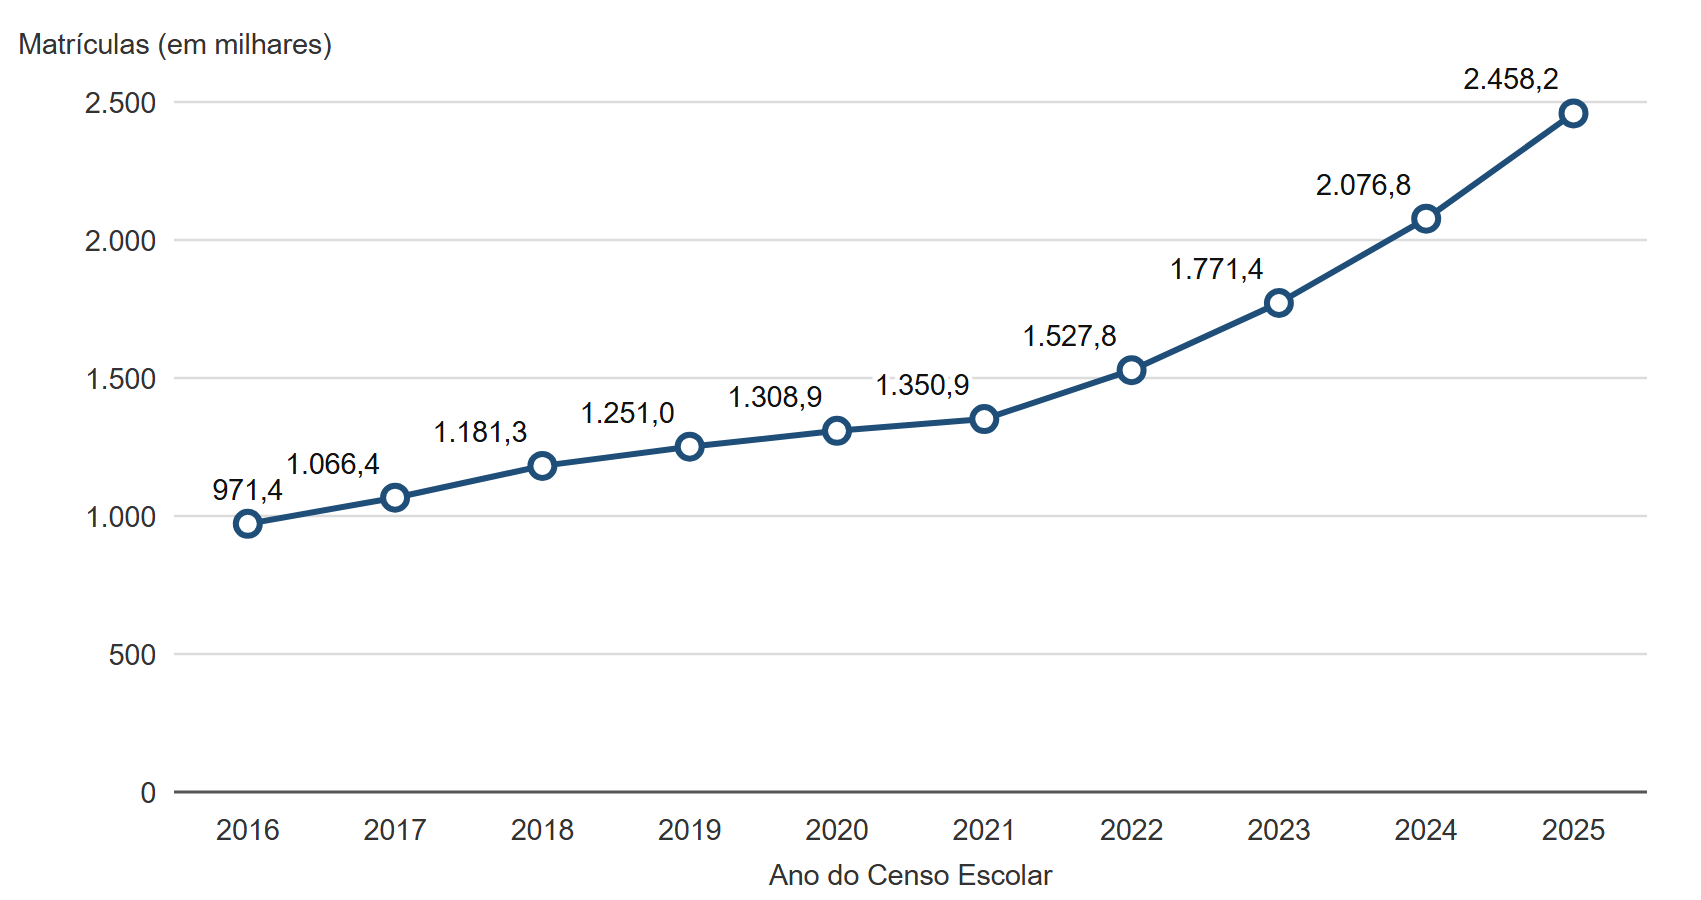
\includegraphics[width=15cm,height=17cm,keepaspectratio]{figuras/grafico01-censo.png}
  \fonte{elaborado pelo autor com base em INEP (2021, p. 22; 2026, p. 24).}
\end{grafico}

Entre 2016 e 2025, as matrículas na educação especial passaram de 971.372 para 2.458.159, um aumento de 153\%. O crescimento acelerou nos últimos anos: de 2016 a 2021, o número subiu 39\%; de 2021 a 2025, subiu 82\%, cerca de 1,1 milhão de matrículas a mais em quatro anos. No mesmo período, a parcela de estudantes de 4 a 17 anos da educação especial incluídos em classes comuns passou de 93,5\% para 96,0\% (INEP, 2026, p. 24). Mais estudantes da educação especial nas classes comuns significa mais planos individualizados para elaborar e, principalmente, para acompanhar, o que aumenta a necessidade de ferramentas que apoiem o professor nesse trabalho.

Os valores de 2016 a 2020 vêm das notas estatísticas do Censo de 2020 (INEP, 2021, p. 22), e os de 2021 a 2025, das notas do Censo de 2025 (INEP, 2026, p. 24). A série de matrículas é comparável: a edição intermediária de 2024 repete os mesmos totais, como os 1.308.900 de 2020 (INEP, 2025, p. 20). O percentual em classes comuns, ao contrário, foi revisado entre edições, com 93,3\% para 2020 na edição de 2021 e 93,2\% na de 2025, e por isso é citado aqui apenas para 2021 a 2025, a partir de uma única edição.

Estar matriculado na classe comum não garante aprendizagem. Para isso, a escola precisa planejar o ensino a partir do que cada estudante já sabe e do que precisa aprender. O Plano Educacional Individualizado (PEI) é o instrumento desse planejamento. Tannús-Valadão e Mendes (2018, p. 11) apontam, entre as funções do PEI, a de registro dos conhecimentos e das habilidades do aluno, “que permite identificar o repertório de partida, acompanhar a evolução em direção às metas e traçar novos caminhos, se determinado programa não estiver permitindo atingir as metas estabelecidas para o estudante”. Com o Decreto nº 12.686/2025, que instituiu a Política Nacional de Educação Especial Inclusiva, e a alteração feita pelo Decreto nº 12.773/2025, passou a ser obrigatório um “documento individualizado de natureza pedagógica, com atualização contínua”, como o Plano de Atendimento Educacional Especializado (PAEE) e o PEI, derivado do estudo de caso do estudante (BRASIL, 2025a, art. 12).

A expressão “atualização contínua” expõe o ponto mais frágil do PEI: o acompanhamento. Tannús-Valadão e Mendes (2018, p. 1, 11-12) relatam um levantamento anterior, feito por Tannús-Valadão em 200 planos de Atendimento Educacional Especializado (AEE) de um município paulista, cujo preenchimento parecia ser feito “por mera formalidade”, com repetições, incoerências e plano formalizado para apenas um terço dos alunos; ao comparar o Brasil com outros países, as autoras concluem que, embora se anuncie a inclusão escolar, “as práticas de planejamento não mudaram”. Sem registros frequentes do desempenho, a revisão do plano depende da memória do professor e de impressões gerais, o que torna difícil dizer se uma meta foi alcançada ou se a estratégia precisa mudar.

Em sua dissertação de mestrado, a pesquisadora Priscila Rodrigues Cruz Francisco enfrentou parte desse problema com o AppPEI (FRANCISCO, 2023), um recurso educacional digital construído em planilha eletrônica, que conduz o professor pelas etapas de elaboração do PEI: dados do aluno, avaliação diagnóstica, matriz de habilidades em quatro áreas, priorização e proposta de intervenção. Na avaliação feita com professores do Colégio de Aplicação da Universidade do Estado do Rio de Janeiro (UERJ), 75\% dos respondentes consideraram o recurso intuitivo, a nota média foi 8,25 e os participantes sugeriram trocar a planilha por uma página web, com navegação mais simples e uso no celular (FRANCISCO, 2023). O AppPEI organiza o planejamento, mas não mede o desempenho do aluno nas habilidades planejadas; a verificação da evolução continua fora da ferramenta.

Este trabalho apresenta o UNIA (Unir Necessidades Individuais e Aprendizagem), um sistema web que parte da estrutura do AppPEI e acrescenta a medição. O nome também remete ao verbo unir: o sistema une as metas do PEI, definidas a partir das necessidades de cada aluno, à medição da aprendizagem nas sessões. O professor cadastra o aluno, o estudo de caso e as metas do PEI; o aluno responde a mini games na tela; o sistema confere cada resposta, classifica o nível de suporte de cada sessão com os mesmos três níveis do AppPEI e mostra a evolução de cada meta em indicadores e gráficos. A revisão do plano passa a contar com uma série de sessões medidas, e não só com a impressão de quem acompanha o aluno.

A pergunta que orienta o trabalho é: como um sistema web pode apoiar o professor no acompanhamento das metas do PEI, medindo de forma automática o desempenho do aluno em atividades digitais e mostrando a evolução ao longo do tempo?

\section{Justificativa}\label{sec:1.1}

A primeira razão é normativa. A Resolução nº 4/2009 do Conselho Nacional de Educação, Câmara de Educação Básica (CNE/CEB), atribui ao professor do AEE a elaboração e a execução do plano de AEE, avaliando a funcionalidade e a aplicabilidade dos recursos pedagógicos, e o acompanhamento desses recursos na sala de aula comum (BRASIL, 2009, art. 13). A Lei Brasileira de Inclusão inclui, entre os deveres do poder público, o planejamento de estudo de caso, a elaboração de plano de atendimento educacional especializado e a usabilidade pedagógica de recursos de tecnologia assistiva (BRASIL, 2015, art. 28, VII). A norma de 2025 reforça essas atribuições ao exigir atualização contínua do PAEE e do PEI (BRASIL, 2025a, art. 12), e a Portaria nº 421/2026 do Ministério da Educação (MEC), que a regulamenta, inclui entre os conteúdos mínimos do PEI “as estratégias de acompanhamento e de monitoramento do plano” (BRASIL, 2026, art. 11, III). Acompanhar exige registros, e registros feitos à mão a cada sessão consomem um tempo que o professor raramente tem.

A segunda razão é a lacuna nas ferramentas. Francisco (2023) não encontrou aplicativos de PEI na loja Google Play. Nas fontes consultadas nesta pesquisa (seção~\ref{sec:2.5}), as ferramentas digitais tratam ou da elaboração e do registro do PEI ou de jogos para a aprendizagem; não se encontrou uma que associe o desempenho medido nos jogos às metas do plano. Um sistema com essa ligação também atende ao pedido dos professores que avaliaram o AppPEI, que sugeriram um formato web acessível pelo celular.

A terceira razão é pedagógica. O PEI existe para que o aluno avance em direção à autonomia, isto é, para que passe a realizar sozinho o que antes realizava com ajuda. Esse movimento corresponde à passagem entre os níveis “realiza com ajuda” e “realiza sem necessidade de suporte” do AppPEI e, na teoria histórico-cultural, à ideia de que aquilo que a criança faz hoje com assistência ela fará sozinha amanhã (VIGOTSKI, 2007). Tornar essa passagem visível, sessão após sessão, ajuda o professor a decidir quando retirar o apoio e quando mudar a estratégia.

\section{Objetivos}\label{sec:1.2}

\subsection{Objetivo geral}\label{sec:1.2.1}

Desenvolver um sistema web que apoie o professor no acompanhamento das metas do PEI de alunos da educação especial dos anos iniciais, medindo de forma automática o desempenho em mini games e apresentando a evolução de cada meta.

\subsection{Objetivos específicos}\label{sec:1.2.2}

\begin{alineasIFTO}
  \item identificar, na legislação e na literatura, os elementos do PEI e os níveis de suporte usados para acompanhar metas, tomando o AppPEI como referência;
  \item modelar e implementar o cadastro de alunos, do estudo de caso e das metas por área, com nível de suporte inicial e data de revisão;
  \item desenvolver mini games que registrem acerto, uso de dica e tempo de resposta nas quatro áreas da matriz do AppPEI;
  \item definir uma regra de classificação do nível de suporte por sessão e indicadores de evolução por meta, apresentados em tabelas e gráficos acessíveis;
  \item verificar o funcionamento e a usabilidade do sistema por meio de testes automatizados, de um teste de ponta a ponta e de uma avaliação heurística.
\end{alineasIFTO}

\section{Estrutura do trabalho}\label{sec:1.3}

Além desta introdução, o trabalho tem cinco capítulos. O capítulo~\ref{cap:2} reúne a fundamentação teórica: a educação especial na perspectiva inclusiva e seu marco legal, o PEI e os níveis de suporte, a medição frequente do progresso, os jogos digitais na educação e os trabalhos relacionados. O capítulo~\ref{cap:3} descreve a metodologia da pesquisa e do desenvolvimento. O capítulo~\ref{cap:4} apresenta o UNIA: requisitos, arquitetura, modelo de dados, mini games, regras de medição, gráficos, segurança e acessibilidade. O capítulo~\ref{cap:5} discute a verificação técnica, compara o UNIA com o AppPEI, relata a avaliação heurística e expõe as limitações. O capítulo~\ref{cap:6} traz as considerações finais e os trabalhos futuros.

% Gerado de tcc.md (exportado do Claude Docs) por ferramentas/gera_latex.php em 12/11/2026 21:45.
% Para mudar o texto, edite este arquivo; se gerar de novo a partir do documento, as edições feitas aqui se perdem.

\chapter{FUNDAMENTAÇÃO TEÓRICA}\label{cap:2}

Este capítulo reúne os conceitos que sustentam o UNIA. As seções~\ref{sec:2.1} a~\ref{sec:2.3} tratam do direito à educação inclusiva, do PEI e dos níveis de suporte; as seções~\ref{sec:2.4} e~\ref{sec:2.5}, da medição do progresso, dos jogos digitais e dos trabalhos relacionados.

\section{Educação especial na perspectiva inclusiva}\label{sec:2.1}

A Constituição Federal garante o atendimento educacional especializado às pessoas com deficiência, preferencialmente na rede regular de ensino (BRASIL, [2026], art. 208, III). A Lei de Diretrizes e Bases da Educação Nacional (LDB) define a educação especial como modalidade escolar oferecida preferencialmente na rede regular e obriga os sistemas de ensino a assegurar currículos, métodos, técnicas e recursos educativos específicos para atender às necessidades desses educandos (BRASIL, 1996, arts. 58 e 59).

A Política Nacional de Educação Especial na Perspectiva da Educação Inclusiva, de 2008, deslocou o foco da escola especial para a classe comum: o AEE passou a complementar ou suplementar a escolarização, e não a substituí-la (BRASIL, 2008). O Decreto nº 7.611/2011 descreve o AEE como um conjunto de atividades e de recursos pedagógicos e de acessibilidade organizados de forma institucional e contínua (BRASIL, 2011), e a Resolução CNE/CEB nº 4/2009 atribui ao professor do AEE a elaboração, a execução e a avaliação do plano de AEE (BRASIL, 2009, art. 13).

A Lei Brasileira de Inclusão (LBI) ampliou esse quadro. Ela assegura um sistema educacional inclusivo em todos os níveis (BRASIL, 2015, art. 27) e inclui entre os deveres do poder público o planejamento de estudo de caso, a elaboração de plano de atendimento educacional especializado e a usabilidade pedagógica de recursos de tecnologia assistiva (BRASIL, 2015, art. 28, VII). A mesma lei define tecnologia assistiva como produtos, recursos, metodologias, estratégias, práticas e serviços que promovem a funcionalidade da pessoa com deficiência, com vistas à sua autonomia e inclusão (BRASIL, 2015, art. 3º, III).

Entre 2025 e 2026, três normas reorganizaram esse campo. O Decreto nº 12.686/2025 instituiu a Política Nacional de Educação Especial Inclusiva (PNEEI), voltada a estudantes com deficiência, com transtorno do espectro autista (TEA) e com altas habilidades ou superdotação (BRASIL, 2025a, art. 1º). O decreto adota o estudo de caso como “metodologia de produção, sistematização e registro de informações” sobre o estudante (BRASIL, 2025a, art. 11) e determina que a oferta do AEE não seja condicionada a diagnóstico ou laudo (BRASIL, 2025a, art. 11, § 7º). O Decreto nº 12.773/2025 alterou o texto para que o resultado do estudo de caso fundamente tanto o PAEE quanto o PEI, documentos obrigatórios e de atualização contínua (BRASIL, 2025b). Por fim, a Portaria MEC nº 421/2026 regulamentou a política, definiu o conteúdo mínimo de cada documento e determinou que o PAEE e o PEI sejam “revisados anualmente, de modo a compatibilizá-los com a avaliação contínua do estudante” (BRASIL, 2026, art. 7º, § 3º).

Três pontos dessas normas orientam este trabalho: o PEI deriva do estudo de caso, deve ser atualizado de forma contínua e precisa prever como o plano será acompanhado. O capítulo~\ref{cap:4} mostra como o UNIA trata cada um deles.

\section{Plano Educacional Individualizado}\label{sec:2.2}

O PEI é o registro do planejamento feito para um estudante específico. Tannús-Valadão e Mendes (2018) o descrevem como, ao mesmo tempo, um documento que especifica o programa educacional de um estudante a partir de seus pontos fortes e necessidades, um registro das diferenciações de que ele precisa para alcançar as expectativas de aprendizagem e um instrumento de prestação de contas ao aluno, à família e à equipe. Não se trata de um currículo paralelo: o plano parte do currículo comum e indica os apoios de que o aluno precisa para participar dele.

Francisco (2023) organiza o planejamento educacional individualizado em cinco etapas, que se repetem em ciclo:

\begin{passos}
  \item Identificação do estudante e de suas necessidades.
  \item Avaliação das habilidades que o estudante já realiza.
  \item Estruturação do plano, com as habilidades priorizadas e as estratégias.
  \item Aplicação das atividades planejadas.
  \item Avaliação e replanejamento, com a revisão do plano a partir dos resultados.
\end{passos}

As duas últimas etapas são as que mais dependem de registros. É nelas que se verifica se a habilidade priorizada avançou e se a estratégia deve mudar. Tannús-Valadão e Mendes (2018, p. 13) observam que estudos feitos na França, na Espanha, na Itália e nos Estados Unidos indicam efeitos positivos do uso do PEI e, principalmente, de seus critérios de acompanhamento, como a avaliação e a reavaliação do processo de escolarização.

A literatura aponta, porém, que essas etapas nem sempre se completam. Em 2018, Tannús-Valadão e Mendes constatavam que o Brasil não tinha dispositivos na legislação federal que garantissem um PEI baseado nas peculiaridades de cada estudante e que, na prática, o planejamento se concentrava nos serviços da sala de recursos multifuncionais, sem relação com o ensino na classe comum. As normas de 2025 e 2026, descritas na seção~\ref{sec:2.1}, passaram a exigir o PEI, mas a exigência, sozinha, não garante que o plano seja acompanhado. Um plano que não é revisto com base em dados tende a virar documento de arquivo.

A Portaria MEC nº 421/2026 deu forma a esse instrumento. Pelo art. 11, o PEI “contempla o plano de acessibilização curricular” e deve conter, no mínimo (BRASIL, 2026, art. 11):

\begin{alineasIFTO}
  \item as atividades a serem desenvolvidas na sala de recursos multifuncionais ou em outros espaços do AEE e sua articulação com o professor regente;
  \item as medidas de acessibilidade curricular, didático-pedagógica e avaliativa indicadas pelo estudo de caso;
  \item as estratégias de acompanhamento e de monitoramento do plano;
  \item o registro das devolutivas às famílias.
\end{alineasIFTO}

A norma exige estratégias de acompanhamento e de monitoramento, mas não diz como executá-las. É nesse ponto que um sistema pode ajudar, ao transformar a aplicação das atividades em registros que se acumulam e podem ser comparados.

\section{Níveis de suporte e autonomia}\label{sec:2.3}

Para registrar o que o aluno já realiza, o AppPEI usa um inventário de habilidades em que cada habilidade recebe um de três níveis: “não realiza”, “realiza com ajuda” e “realiza sem necessidade de suporte” (FRANCISCO, 2023). Os níveis dizem mais do que acerto ou erro: indicam quanto apoio o aluno precisa para chegar ao resultado.

Essa gradação tem base na teoria histórico-cultural. Vigotski (2007) distingue o nível de desenvolvimento real, expresso no que a criança resolve sozinha, do nível de desenvolvimento potencial, expresso no que ela resolve com a orientação de um adulto ou em colaboração com um colega mais capaz. A distância entre os dois é a zona de desenvolvimento proximal, e o que hoje a criança faz com ajuda tende a ser feito por ela sozinha mais tarde. Nessa leitura, a habilidade em “realiza com ajuda” é justamente aquela em que o ensino deve atuar, e a passagem para “realiza sem necessidade de suporte” é o sinal de que o apoio pode ser retirado.

No UNIA, a ajuda oferecida na tela é a dica: quando o aluno a pede, o sistema elimina opções e deixa apenas duas, uma delas a correta. Por ser um apoio padronizado, a dica pode ser contada, e a frequência com que o aluno a usa ao longo das sessões indica o quanto ele ainda depende de suporte. Trata-se de uma simplificação: em sala, a ajuda assume várias formas (verbal, gestual, física), e o sistema registra apenas a que ele próprio oferece. A regra que transforma acertos e dicas em níveis está na seção~\ref{sec:4.5}.

\section{Medição frequente do progresso e jogos digitais}\label{sec:2.4}

Saber se uma meta avança exige medir a mesma habilidade várias vezes, da mesma forma, e comparar os resultados. Deno (1985) propôs essa lógica na medida baseada no currículo (\textit{curriculum-based measurement}): provas curtas, aplicadas com frequência sobre as habilidades que estão sendo ensinadas, cujos resultados são lançados em gráfico para que o professor veja a tendência e decida se mantém ou muda o ensino. A proposta surgiu na educação especial como alternativa intermediária entre os testes padronizados e a observação informal, reunindo vantagens de ambos (DENO, 1985).

O UNIA segue essa lógica em escala reduzida. Cada sessão tem cinco rodadas sobre uma habilidade da meta, o resultado é gravado com data e as sessões de uma meta formam uma série que o sistema transforma em indicadores e gráficos. A diferença é que, no UNIA, quem aplica e corrige a prova é o próprio sistema.

Os jogos digitais são um meio adequado para isso. Prensky (2012) destaca que os jogos combinam envolvimento com retorno imediato: o jogador age, vê o resultado e tenta de novo. Para a medição, interessa uma propriedade adicional. Numa atividade digital, cada resposta pode ser registrada no momento em que acontece, com o acerto, o tempo e o apoio usado, sem trabalho extra do professor; no papel, o mesmo registro exigiria anotar cada tentativa durante a atividade.

Há dois limites a considerar. O primeiro é que o jogo mede o desempenho naquele jogo, e a transferência da habilidade para outras situações ainda precisa ser observada pelo professor. O segundo é que todo jogo depende dos sentidos e dos movimentos que exige: uma atividade que pede para ver figuras e tocá-las não mede da mesma forma o desempenho de uma criança com baixa visão ou com dificuldade motora. Esses limites voltam no capítulo~\ref{cap:5}.

\section{Trabalhos relacionados}\label{sec:2.5}

Os trabalhos relacionados foram localizados por uma busca estruturada, feita em 9 de novembro de 2026 e guiada por uma pergunta: que recursos digitais apoiam o PEI ou o ensino de estudantes com deficiência ou TEA na educação básica, e esses recursos registram o desempenho do estudante e o ligam às metas do plano? Foram consultadas três bases, sem limite de ano:

\begin{alineasIFTO}
  \item Biblioteca Digital Brasileira de Teses e Dissertações (BDTD), pela busca da própria base, em todos os campos: “plano educacional individualizado” aplicativo (19 resultados), “plano educacional individualizado” sistema digital (6) e “jogos digitais” “educação especial” alfabetização (6);
  \item SBC OpenLib, biblioteca digital da Sociedade Brasileira de Computação (SBC), por buscador da web restrito aos endereços da base: plano educacional individualizado sistema aplicativo (9 trabalhos) e jogo digital alfabetização crianças deficiência intelectual autismo desempenho professor acompanhamento (9);
  \item Scientific Electronic Library Online (SciELO), por buscador da web restrito ao endereço da base: plano educacional individualizado tecnologia digital aplicativo (7) e jogos digitais educação especial alfabetização matemática avaliação desempenho (5).
\end{alineasIFTO}

Descartados os resultados repetidos e os de fora das bases, restaram 57 trabalhos: 27 da BDTD, 18 da SBC OpenLib e 12 da SciELO. Leram-se o título e o resumo de cada um e, quando o resumo não bastou, o texto completo. Foram incluídos os trabalhos que desenvolvem um recurso digital (sistema, aplicativo ou jogo) voltado à educação básica e destinado a estudantes com deficiência ou TEA, ou à elaboração e ao acompanhamento do PEI. Foram excluídos os estudos sem recurso digital, que eram a maioria e tratavam de formação docente, legislação e prática pedagógica; os que avaliam jogos prontos, sem desenvolvê-los; os que oferecem material de apoio em vez de um recurso usado com o estudante ou com o PEI, como um e-book de estratégias, um repositório de orientações para professores e um modelo para quem desenvolve jogos; os voltados ao ensino superior, a rotinas diárias ou a estudantes fora da educação especial; os que não informam o público ou o conteúdo trabalhado; e um artigo cujo texto estava indisponível no dia da busca. Dez trabalhos atenderam aos critérios, cinco da BDTD e cinco da SBC OpenLib. Nenhum veio da SciELO, cujos resultados discutiam o PEI e a prática docente ou usavam jogos prontos ou não digitais. A eles se somaram dois trabalhos conhecidos antes da busca: o ABC Autismo, que atende aos mesmos critérios, e o sistema descrito na revista Temática, que gere os PEIs dos estudantes do IFRN, inclusive os dos cursos técnicos integrados ao ensino médio. Os doze trabalhos formam dois grupos: ferramentas para o PEI, a começar pelo AppPEI, e jogos ou aplicativos usados pelo estudante.

Priscila Rodrigues Cruz Francisco desenvolveu o AppPEI no Mestrado Profissional em Ensino na Educação Básica do Instituto de Aplicação Fernando Rodrigues da Silveira (CAp-UERJ). O recurso foi construído em planilha eletrônica do Google e tem nove menus: capa, informações, menu inicial, alunos, professores, avaliação diagnóstica, matriz e priorização de habilidades, proposta e PEI completo. A matriz de habilidades, construída pela autora a partir de referências da área, divide-se em quatro áreas: Alfabetização Matemática, Comunicação Oral, Leitura e Escrita e Alfabetização Digital. Cinco professores do colégio participaram da avaliação; quatro responderam ao questionário e três concluíram um PEI. Metade considerou o acesso fácil, 75\% consideraram o recurso intuitivo e a nota média foi 8,25. As sugestões incluíram migrar para páginas em HyperText Markup Language (HTML), melhorar a navegação e o layout, permitir o uso no celular e deixar o professor editar a matriz de habilidades (FRANCISCO, 2023).

Dois trabalhos da busca também tratam o PEI como documento digital. Almeida (2023) acompanhou professores do ensino comum e da educação especial na elaboração do PEI de um aluno autista, numa escola de Balsas, no Maranhão, e propôs como produto o PEI-DIGITAL, aplicativo de uso interno da escola que os professores podem preencher em conjunto depois de definir os objetivos, as metas, as estratégias e as adaptações curriculares do plano. Diniz \textit{et al.} (2024, p. 107-109) apresentaram o PAR Digital, sigla de Planejar, Aplicar, Rever: um sistema web para preencher e gerir o PEI de estudantes com deficiência em classes comuns, com um banco de estratégias baseadas no Desenho Universal para a Aprendizagem. O professor cadastra as estratégias do plano e marca a situação de cada uma, como alcançada ou não alcançada, e o sistema gera relatórios de progresso por disciplina; segundo os autores, a ferramenta foi validada e usada por escolas da educação básica.

Paiva \textit{et al.} (2026) desenvolveram, por pesquisa-ação e em parceria com o Núcleo de Apoio às Pessoas com Necessidades Educacionais Específicas (NAPNE) do Instituto Federal do Rio Grande do Norte (IFRN), Campus Pau dos Ferros, um sistema web para gerir os PEIs dos estudantes da instituição. O PEI é criado automaticamente quando o estudante é incluído na oferta de uma disciplina; o professor registra os objetivos, os conteúdos, as metodologias e os recursos adaptados, e o plano passa pelas situações não iniciado, em andamento, preenchido e finalizado. O acompanhamento é feito pelos pareceres pedagógicos de cada bimestre ou semestre, pelas notas, pelo histórico do estudante e por comentários da equipe (PAIVA \textit{et al.}, 2026, p. 65, 69-73). Na avaliação pelo Modelo de Aceitação de Tecnologia, os 10 profissionais participantes concordaram, total ou parcialmente, que aprender a usar o sistema é fácil (PAIVA \textit{et al.}, 2026, p. 78). O trabalho mostra que a demanda por apoio digital ao PEI também aparece na rede federal.

O segundo grupo reúne jogos e aplicativos usados pelo estudante. Farias, Silva e Cunha (2014), do Instituto Federal de Alagoas (IFAL), desenvolveram o ABC Autismo, aplicativo móvel que apoia a alfabetização de crianças com autismo com base nas premissas do programa Treatment and Education of Autistic and Related Communication Handicapped Children (TEACCH); a validação com crianças, pais e profissionais de uma associação indicou alinhamento ao programa e interface autoexplicativa. Negrim (2019) desenvolveu um jogo digital de alfabetização e o usou com cinco alunos com deficiência intelectual do ensino fundamental; avaliações diagnósticas feitas ao longo das fases do jogo apontaram avanços nas hipóteses de escrita da maioria deles. Bentes, Araújo e Pires (2020) criaram o ANE, aplicativo de jogos para que crianças com deficiência intelectual aprendam o alfabeto, os numerais e as emoções, com requisitos levantados a partir de dados do atendimento educacional especializado de um município; nos testes com usuários finais, todos o consideraram boa ferramenta de apoio para responsáveis e profissionais da educação especial. Dutra, Maschio e Gasparini (2023) desenvolveram o Pensar e Lavar, jogo acessível de pensamento computacional para crianças neurotípicas e com deficiência intelectual no início da alfabetização, avaliado em quatro etapas, uma delas com 47 crianças.

Galdino (2024, p. 61, 66) criou um site com jogos digitais de alfabetização matemática para alunos com TEA, como os de sequência numérica e de quantidade, feitos no PowerPoint para que o professor possa editá-los e adaptá-los a cada aluno. Silva, Santos e Cunha (2024), também do IFAL, apresentaram o LetraMundo, jogo sério web para a alfabetização de crianças com TEA em ambiente escolar; no teste preliminar, profissionais da educação especial apontaram a necessidade de redistribuir os níveis de dificuldade e de criar atividades com grafemas. Mesquita e Bastos (2025) descreveram o Garimpeirinhos, ambiente web de apoio à alfabetização e à inclusão na educação infantil e nos anos iniciais, com jogos, leitura progressiva, prancha de comunicação alternativa e utilitários para o professor. Fernandes (2026) desenvolveu cinco jogos no Scratch para a alfabetização de estudantes com TEA, com foco em consciência fonológica, relação entre grafema e fonema e sequência alfabética; a avaliação, qualitativa, apontou mais engajamento e mais tempo de atenção durante as tarefas.

\begin{tabelaIFTO}
\setlength{\largtab}{\dimexpr\linewidth-10\tabcolsep-6\arrayrulewidth-1pt\relax}
\begin{longtable}{|L{0.2253}|L{0.16}|L{0.2253}|L{0.2008}|L{0.1885}|}
\legendatab{quadro}{Trabalhos relacionados e o UNIA}{qua:1}{5}\\
\hline
\textbf{Trabalho} & \textbf{Recurso} & \textbf{Público e foco} & \textbf{Registro do desempenho} & \textbf{Ligação com as metas do PEI} \\
\hline
\endfirsthead
\multicolumn{5}{@{}r@{}}{\textit{(continuação)}}\\
\hline
\textbf{Trabalho} & \textbf{Recurso} & \textbf{Público e foco} & \textbf{Registro do desempenho} & \textbf{Ligação com as metas do PEI} \\
\hline
\endhead
\multicolumn{5}{@{}r@{}}{\textit{(continua)}}\\
\endfoot
\fontetab{5}{elaboração própria (2026), com base nos trabalhos citados. “Não relatado” e “Não abordada” indicam que o tema não aparece no texto consultado de cada trabalho.}
\endlastfoot
AppPEI (FRANCISCO, 2023) & Planilha eletrônica & Professores; elaboração do PEI & Avaliação diagnóstica preenchida pelo professor & Monta o PEI a partir das habilidades priorizadas \\ \hline
PEI-DIGITAL (ALMEIDA, 2023) & Aplicativo & Professores; elaboração do PEI em conjunto & Não relatado & Registra objetivos, metas e estratégias do plano \\ \hline
PAR Digital (DINIZ \textit{et al.}, 2024) & Sistema web & Professores e coordenadores; gestão do PEI & Situação de cada estratégia, marcada pelo professor, e relatórios & Estratégias e relatórios ficam no PEI \\ \hline
Sistema de gestão de PEIs do NAPNE/IFRN (PAIVA \textit{et al.}, 2026) & Sistema web & Professores, pedagogos e coordenação; elaboração e gestão do PEI por disciplina & Pareceres por bimestre ou semestre e notas, lançados pela equipe & Objetivos, conteúdos e métodos adaptados ficam no PEI; o progresso não é medido por meta \\ \hline
ABC Autismo (FARIAS; SILVA; CUNHA, 2014) & Aplicativo móvel & Crianças com TEA; alfabetização & Não relatado & Não abordada \\ \hline
Jogo de alfabetização (NEGRIM, 2019) & Jogo digital & Alunos com deficiência intelectual; leitura e escrita & Avaliações diagnósticas ao longo das fases do jogo & Não abordada \\ \hline
ANE (BENTES; ARAÚJO; PIRES, 2020) & Aplicativo de jogos & Crianças com deficiência intelectual; alfabeto, numerais e emoções & Não relatado & Não abordada \\ \hline
Pensar e Lavar (DUTRA; MASCHIO; GASPARINI, 2023) & Jogo digital & Crianças com e sem deficiência intelectual; pensamento computacional & Não relatado & Não abordada \\ \hline
Jogos de alfabetização matemática (GALDINO, 2024) & Site com jogos feitos no PowerPoint & Alunos com TEA; alfabetização matemática & Não relatado & Discutida no texto, não nos jogos \\ \hline
LetraMundo (SILVA; SANTOS; CUNHA, 2024) & Jogo web & Crianças com TEA; alfabetização na escola & Não relatado & Não abordada \\ \hline
Garimpeirinhos (MESQUITA; BASTOS, 2025) & Ambiente web & Educação infantil e anos iniciais, com recursos para TEA; alfabetização & Não relatado & Não abordada \\ \hline
Jogos em Scratch (FERNANDES, 2026) & Jogos digitais & Estudantes com TEA; consciência fonológica e alfabeto & Observação e registros das professoras & Não abordada \\ \hline
UNIA (este trabalho) & Sistema web & Professor e aluno dos anos iniciais; metas do PEI & Acertos, erros, dicas e tempo de cada sessão, gravados pelo sistema & Cada sessão medida entra no histórico da meta \\ \hline
\end{longtable}
\end{tabelaIFTO}

O Quadro~\ref{qua:1} mostra dois grupos. As ferramentas do primeiro organizam o PEI como documento. A mais próxima do UNIA é o PAR Digital, que liga as estratégias ao plano e gera relatórios de progresso, mas o andamento depende do que o professor marca em cada estratégia (DINIZ \textit{et al.}, 2024, p. 109). No sistema do NAPNE/IFRN, o progresso também depende do que a equipe registra: os pareceres de cada bimestre ou semestre e as notas (PAIVA \textit{et al.}, 2026, p. 70, 72). Os jogos do segundo grupo trabalham as habilidades com o estudante; nos que relatam algum acompanhamento, ele vem de avaliações da pesquisa ou da observação das professoras, e nenhum liga o desempenho às metas de um plano individualizado. Fernandes (2026) recomenda, como próximo passo, incorporar métricas padronizadas de aprendizagem e registrar de forma sistemática o progresso dos estudantes. O UNIA junta as duas partes: os mini games existem para medir as metas do PEI, o próprio sistema grava o desempenho do aluno em cada sessão, e cada resultado entra no histórico da meta correspondente.

% Gerado de tcc.md (exportado do Claude Docs) por ferramentas/gera_latex.php em 12/11/2026 21:45.
% Para mudar o texto, edite este arquivo; se gerar de novo a partir do documento, as edições feitas aqui se perdem.

\chapter{METODOLOGIA}\label{cap:3}

Este capítulo classifica a pesquisa e descreve como o UNIA foi desenvolvido e verificado.

\section{Classificação da pesquisa}\label{sec:3.1}

Quanto à natureza, a pesquisa é aplicada, pois busca gerar conhecimento para resolver um problema prático e específico: o acompanhamento das metas do PEI (PRODANOV; FREITAS, 2013). Quanto aos objetivos, é exploratória, porque trata de um tema com poucos trabalhos que liguem o PEI à medição automática do desempenho e procura torná-lo mais claro por meio da construção de uma solução (GIL, 2017). Quanto aos procedimentos, combina pesquisa bibliográfica, sobre o PEI, os níveis de suporte, a medição do progresso e os jogos digitais; pesquisa documental, sobre a legislação da educação especial; e o desenvolvimento de um artefato de software.

Esse último procedimento aproxima o trabalho da \textit{Design Science Research}, abordagem que orienta a construção e a avaliação de artefatos voltados a problemas reais (DRESCH; LACERDA; ANTUNES JÚNIOR, 2015). Aqui, a avaliação do artefato se limitou à verificação técnica descrita na seção~\ref{sec:3.4}; a avaliação com professores e alunos fica para uma etapa posterior.

\section{Etapas do desenvolvimento}\label{sec:3.2}

O UNIA foi construído de forma incremental, em versões que acrescentaram funcionalidades à anterior e foram revistas a cada entrega (SOMMERVILLE, 2011). O Quadro~\ref{qua:2} resume as três versões.

\begin{tabelacurta}
\setlength{\largtab}{\dimexpr\linewidth-4\tabcolsep-3\arrayrulewidth-1pt\relax}
\legenda{quadro}{Versões do UNIA}\label{qua:2}\vspace{4pt}
\begin{tabular}{|L{0.1506}|L{0.8494}|}
\hline
\textbf{Versão} & \textbf{Principais mudanças} \\
\hline
1 & Catálogo de atividades por tipo de deficiência, login e cadastro de usuários. \\ \hline
2 & Reestruturação no padrão Model-View-Controller (MVC), com roteador central; cadastro de alunos e de metas do PEI, com as áreas e os níveis do AppPEI; registros de acompanhamento; proteção contra Cross-Site Request Forgery (CSRF), consultas parametrizadas e senhas com hash. \\ \hline
3 & Sessões de mini games na tela, com medição automática; catálogo restrito a atividades medidas pelo sistema (24 atividades, seis por área); evolução por meta com indicadores e gráficos. \\ \hline
\end{tabular}
\fonte{elaboração própria (2026).}
\end{tabelacurta}

A versão 3 concentra a contribuição deste trabalho e seguiu cinco passos:

\begin{passos}
  \item Levantamento: leitura da dissertação de Francisco (2023), da legislação e dos trabalhos relacionados, localizados pela busca descrita na seção~\ref{sec:2.5}, para definir as áreas, os níveis de suporte e o que o sistema deveria registrar.
  \item Definição do que medir: escolha das habilidades que podem ser medidas na tela sem depender de anotação do professor.
  \item Modelagem: diagrama de pacotes da arquitetura, diagrama de classes do domínio e diagrama de sequência da sessão, na notação da Unified Modeling Language (UML), versão 2.5.1 (OBJECT MANAGEMENT GROUP, 2017), e modelo lógico do banco de dados na notação pé de galinha (WATT; ENG, 2014), todos desenhados em Scalable Vector Graphics (SVG).
  \item Implementação: banco de dados, regras de medição, mini games, telas e gráficos.
  \item Verificação: testes automatizados, conferência das rotas e teste de ponta a ponta (seção~\ref{sec:3.4}).
\end{passos}

O passo 2 levou a duas decisões que moldaram o sistema. A primeira foi retirar do catálogo as atividades físicas, como as feitas com material concreto, objetos reais, cartões e relevo, porque o resultado delas dependeria de registro manual. A segunda foi não permitir que o professor digite ou edite resultados: todo registro de desempenho nasce de uma sessão medida pelo sistema, e o professor só pode excluir uma sessão feita por engano.

\section{Tecnologias utilizadas}\label{sec:3.3}

O UNIA foi escrito na linguagem PHP: Hypertext Preprocessor (PHP), sem framework. O núcleo que um framework normalmente oferece (roteador, classes-base de controladores e modelos, validação, sessão e proteção contra CSRF) foi implementado no próprio projeto, em classes pequenas, para manter o código legível e sem dependências além do PHPMailer. O código do sistema, sem contar bibliotecas de terceiros, tem 61 arquivos PHP, com cerca de 5.100 linhas, e uma folha de estilo com 285 linhas. O Quadro~\ref{qua:3} lista as tecnologias.

\begin{tabelacurta}
\setlength{\largtab}{\dimexpr\linewidth-4\tabcolsep-3\arrayrulewidth-1pt\relax}
\legenda{quadro}{Tecnologias utilizadas}\label{qua:3}\vspace{4pt}
\begin{tabular}{|L{0.467}|L{0.533}|}
\hline
\textbf{Tecnologia} & \textbf{Uso no UNIA} \\
\hline
PHP 8.2 & Linguagem do servidor, no padrão MVC \\ \hline
MySQL & Banco de dados relacional acessado por PHP Data Objects (PDO); no XAMPP, o servidor é o MariaDB 10.4, compatível com o MySQL \\ \hline
Apache (pacote XAMPP) & Servidor web local, com URLs amigáveis \\ \hline
HTML, Cascading Style Sheets (CSS) e SVG & Telas, figuras dos mini games, gráficos desenhados no servidor e diagramas deste trabalho \\ \hline
Web Speech Application Programming Interface (API) & Voz do navegador no mini game de ouvir a palavra \\ \hline
PHPMailer, via Composer & Envio do e-mail de recuperação de senha \\ \hline
Font Awesome & Ícones da interface \\ \hline
\end{tabular}
\fonte{elaboração própria (2026).}
\end{tabelacurta}

\section{Verificação}\label{sec:3.4}

A verificação teve seis frentes:

\begin{alineasIFTO}
  \item sintaxe: todos os arquivos PHP passaram pela verificação do interpretador (\textit{php -l});
  \item testes automatizados: um script com 63 verificações das regras de negócio cobre a classificação do nível de suporte, as validações dos formulários, a montagem de cada um dos 12 mini games (repetida várias vezes, porque as rodadas são sorteadas), a dica, a meta de destino de cada área, a separação dos resultados por meta, os indicadores de evolução e os gráficos; o script não cobre telas nem banco de dados;
  \item conferência estática: cada uma das 45 rotas aponta para um método existente, e cada classe e método chamado existe;
  \item teste de ponta a ponta: num banco de dados temporário, criado e apagado para o teste, foram cadastrados professor, alunos e metas, executadas seis sessões por área e conferidos a evolução, as sugestões por tipo de deficiência e o cadastro de atividades;
  \item inspeção visual: a ficha do aluno foi renderizada e conferida no navegador, inclusive em largura de tela reduzida;
  \item avaliação heurística: as telas e o código das views foram inspecionados segundo as heurísticas de usabilidade de Nielsen (1994a), e cada problema encontrado recebeu uma nota de severidade de 0 a 4 (NIELSEN, 1994b).
\end{alineasIFTO}

As telas que exigem login ainda dependem de um roteiro de testes manuais, apresentado no Apêndice B. Todos os dados usados nos testes foram fictícios. Como não houve participação de pessoas, a pesquisa não foi submetida a comitê de ética; a avaliação com professores e alunos, prevista como trabalho futuro, exigirá essa submissão e o consentimento dos responsáveis pelas crianças.

% Gerado de tcc.md (exportado do Claude Docs) por ferramentas/gera_latex.php em 12/11/2026 21:45.
% Para mudar o texto, edite este arquivo; se gerar de novo a partir do documento, as edições feitas aqui se perdem.

\chapter{O SISTEMA UNIA}\label{cap:4}

O UNIA é uma aplicação web em que o professor cadastra alunos, registra o estudo de caso e as metas do PEI, aplica sessões de mini games na tela e acompanha a evolução de cada meta. Este capítulo descreve os requisitos, a arquitetura, o modelo de dados, os mini games, as regras de medição, os gráficos, a segurança e a acessibilidade do sistema.

\section{Visão geral e requisitos}\label{sec:4.1}

O sistema tem dois perfis de conta: o professor, que acompanha os próprios alunos, e o administrador, que também mantém a lista de tipos de deficiência. O aluno não tem conta: ele responde às sessões no dispositivo do professor, dentro da sessão aberta por este. O uso típico segue seis passos:

\begin{passos}
  \item O professor cria a conta e entra no sistema.
  \item Cadastra o aluno, com o estudo de caso, o tipo de deficiência, quando informado, e o registro do consentimento do responsável.
  \item Cria as metas do PEI: área, habilidade, nível de suporte inicial e data de revisão.
  \item Escolhe os mini games na ficha do aluno, ou aceita uma sugestão, e entrega o dispositivo ao aluno.
  \item O aluno responde às rodadas, e o sistema grava o resultado na meta.
  \item O professor acompanha a evolução da meta e revisa o plano na data prevista.
\end{passos}

Os Quadros~\ref{qua:4} e~\ref{qua:5} listam os requisitos funcionais (RF) e não funcionais (RNF).

\begin{tabelaIFTO}
\setlength{\largtab}{\dimexpr\linewidth-4\tabcolsep-3\arrayrulewidth-1pt\relax}
\begin{longtable}{|L{0.16}|L{0.84}|}
\legendatab{quadro}{Requisitos funcionais}{qua:4}{2}\\
\hline
\textbf{Código} & \textbf{Requisito} \\
\hline
\endfirsthead
\multicolumn{2}{@{}r@{}}{\textit{(continuação)}}\\
\hline
\textbf{Código} & \textbf{Requisito} \\
\hline
\endhead
\multicolumn{2}{@{}r@{}}{\textit{(continua)}}\\
\endfoot
\fontetab{2}{elaboração própria (2026).}
\endlastfoot
RF01 & Cadastrar professor, entrar e sair do sistema e recuperar a senha por e-mail. \\ \hline
RF02 & Manter os dados da conta, trocar a senha e excluir a própria conta. \\ \hline
RF03 & Cadastrar, editar, listar, buscar e excluir alunos, com estudo de caso, tipo de deficiência e registro do consentimento do responsável. \\ \hline
RF04 & Cadastrar metas do PEI por área, com habilidade, nível de suporte inicial, professor responsável e data de revisão (padrão de 90 dias). \\ \hline
RF05 & Manter o catálogo de atividades, com busca, filtros por tipo de deficiência e por área, paginação, imagem, vídeo, fonte e mini game obrigatório. \\ \hline
RF06 & Sugerir, para cada meta, atividades da mesma área ainda não aplicadas ao aluno e compatíveis com o tipo de deficiência dele. \\ \hline
RF07 & Executar sessões de mini games na tela, com dica e cancelamento, e gravar um registro por meta. \\ \hline
RF08 & Calcular e exibir, por meta, os indicadores de evolução e os gráficos. \\ \hline
RF09 & Exibir o histórico de sessões, com o detalhe por jogo, e permitir excluir um registro feito por engano. \\ \hline
RF10 & Avisar, na tela inicial, as metas com data de revisão vencida. \\ \hline
RF11 & Permitir ao administrador manter os tipos de deficiência. \\ \hline
\end{longtable}
\end{tabelaIFTO}

\begin{tabelacurta}
\setlength{\largtab}{\dimexpr\linewidth-4\tabcolsep-3\arrayrulewidth-1pt\relax}
\legenda{quadro}{Requisitos não funcionais}\label{qua:5}\vspace{4pt}
\begin{tabular}{|L{0.1553}|L{0.8447}|}
\hline
\textbf{Código} & \textbf{Requisito} \\
\hline
RNF01 & Segurança: senhas com hash, consultas parametrizadas, proteção contra CSRF e Cross-Site Scripting (XSS) e controle de acesso por perfil e por dono do dado. \\ \hline
RNF02 & Privacidade: cada professor vê apenas os próprios alunos, e o cadastro registra o consentimento do responsável. \\ \hline
RNF03 & Acessibilidade: práticas inspiradas nas Web Content Accessibility Guidelines (WCAG) 2.1, alvos de toque de pelo menos 44 px e nenhuma informação transmitida só por cor. \\ \hline
RNF04 & Uso em tablet: as sessões funcionam por toque, com botões grandes. \\ \hline
RNF05 & Portabilidade: o sistema roda em servidor PHP com MySQL ou MariaDB, em qualquer pasta do servidor. \\ \hline
RNF06 & Manutenibilidade: código organizado em MVC, com as regras de medição isoladas e cobertas por testes automatizados. \\ \hline
\end{tabular}
\fonte{elaboração própria (2026).}
\end{tabelacurta}

\section{Arquitetura}\label{sec:4.2}

O UNIA segue o padrão MVC, que separa os dados e as regras (Model), a apresentação (View) e o controle do fluxo da requisição (Controller), e o padrão \textit{Front Controller}, em que um único ponto de entrada recebe todas as requisições (FOWLER, 2006). A Figura~\ref{fig:1} mostra a organização do código num diagrama de pacotes da UML.

\begin{figure}[hbp]
  \legendafig{figure}{Diagrama de pacotes do UNIA}{fig:1}
  % Diagrama de pacotes da UML com public, config, core e app (Controllers, Models, Services e Views), ligados por dependências «use» e «instantiate»
  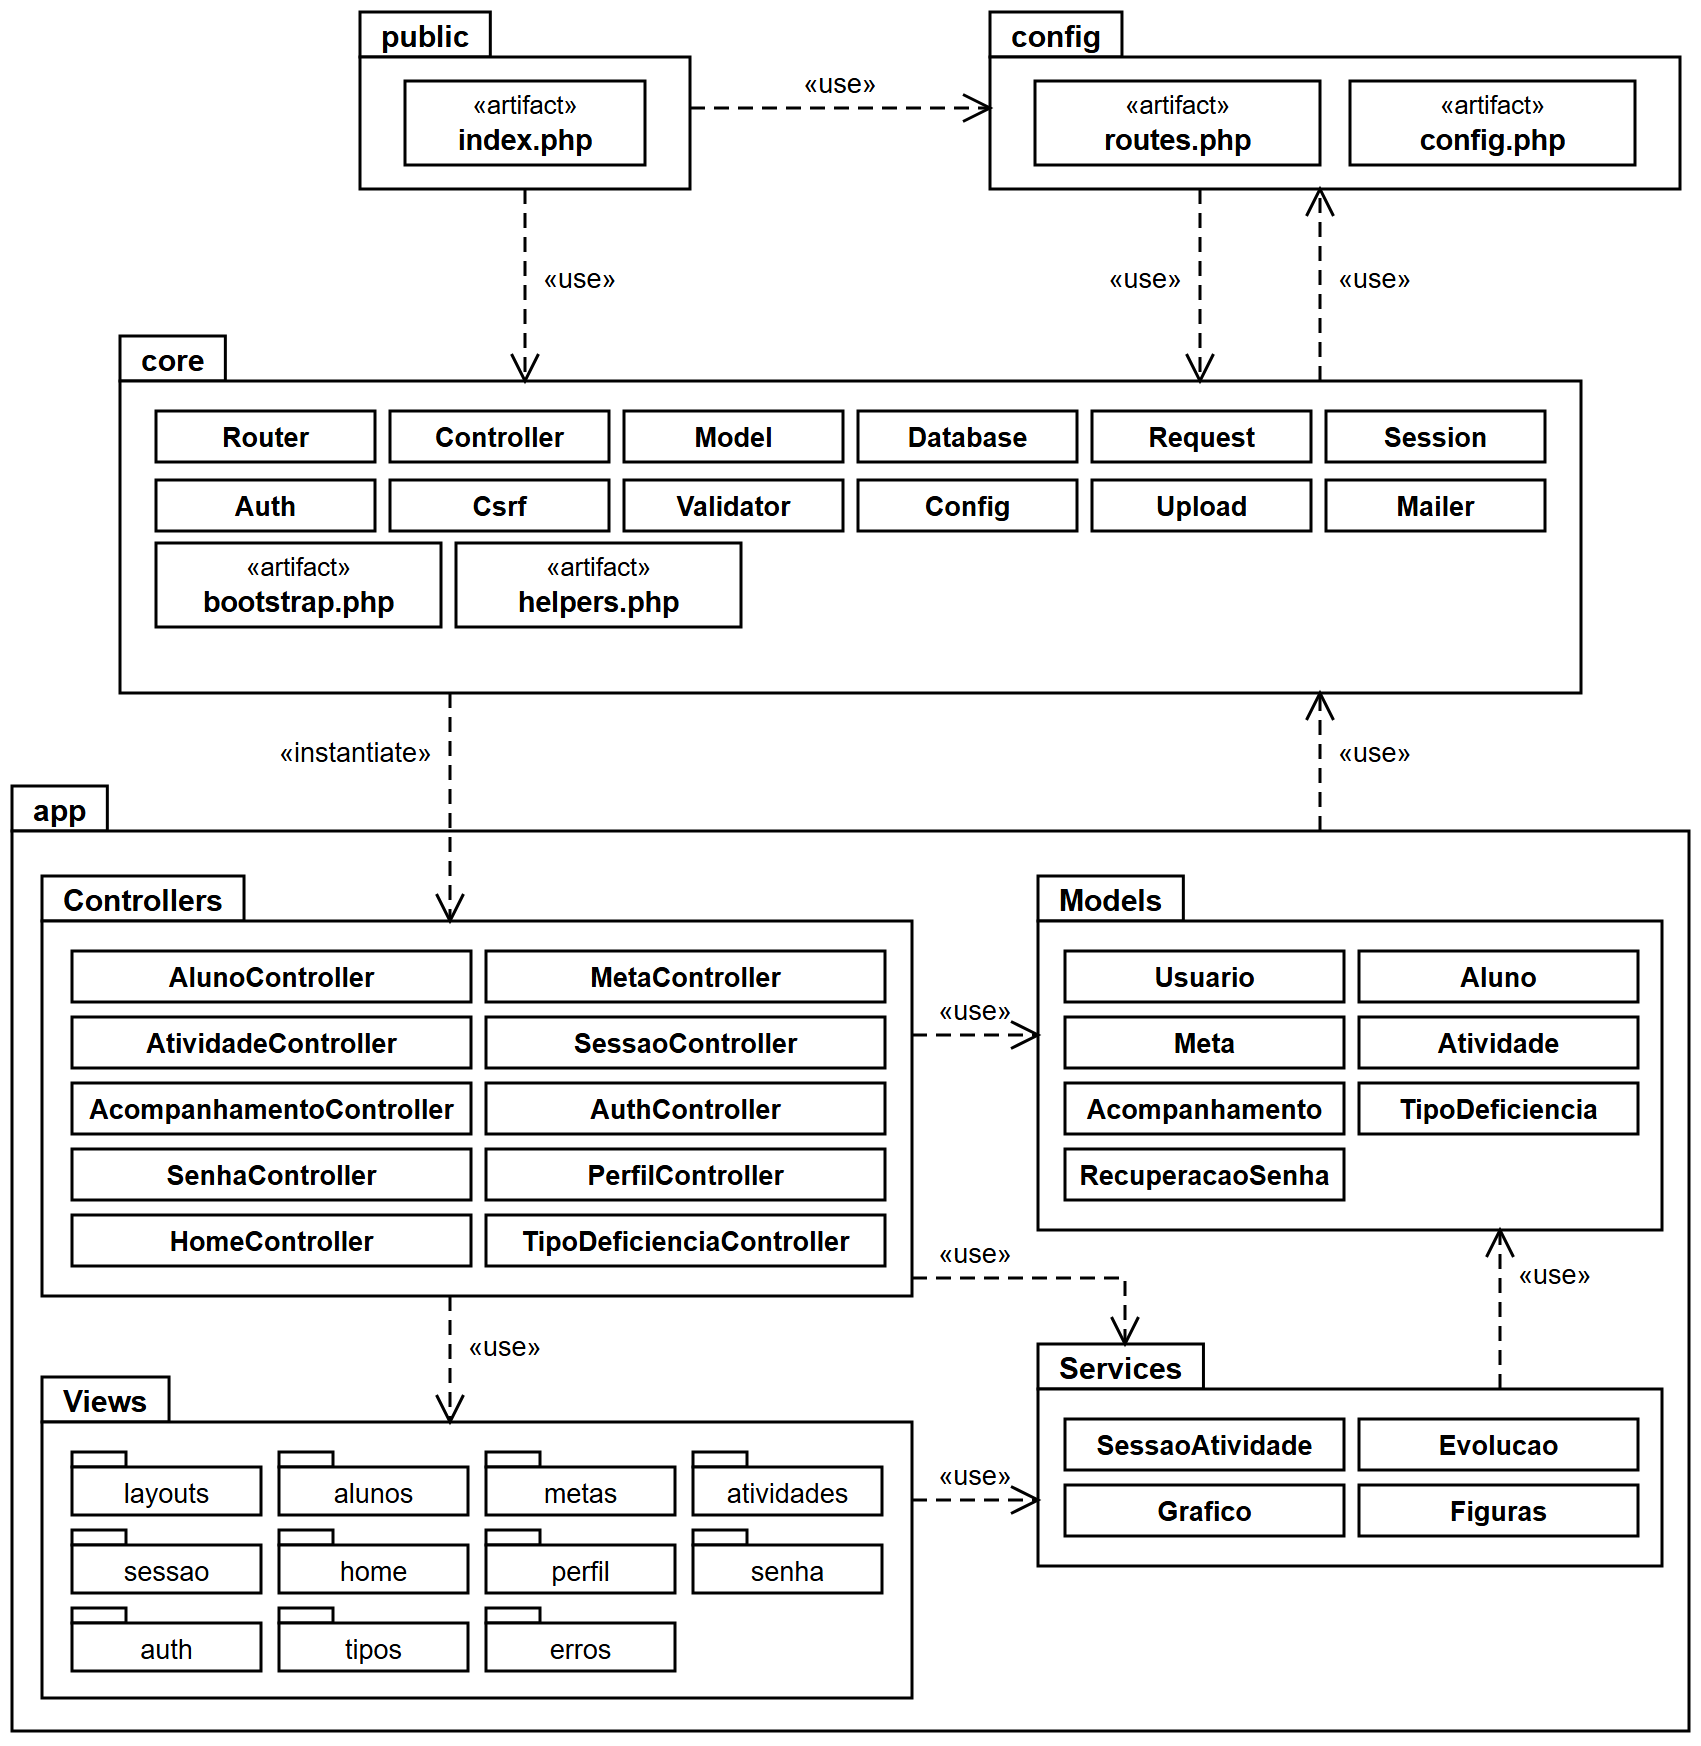
\includegraphics[width=15cm,height=17cm,keepaspectratio]{figuras/figura01-pacotes.png}
  \fonte{elaboração própria (2026).}
\end{figure}

Na notação da UML (OBJECT MANAGEMENT GROUP, 2017, p. 39, 248 e 657), cada pasta do projeto é um pacote, desenhado como um retângulo com uma aba; como os elementos do pacote aparecem dentro dele, o nome fica na aba. As classes aparecem só com o nome, e os arquivos que não são classes, como \textit{index.php} e \textit{routes.php}, aparecem como artefatos, com a palavra-chave «artifact». Cada seta tracejada é uma dependência: o pacote de onde ela sai precisa do pacote para onde ela aponta. A palavra-chave «use» indica que um pacote usa elementos do outro, e «instantiate», que cria instâncias deles, como faz o roteador do núcleo ao criar o controlador de cada requisição. Os pacotes \textit{core} e \textit{config} dependem um do outro, porque \textit{routes.php} cria o roteador e a classe \textit{Config} lê \textit{config.php}. A seta que sai de \textit{app} resume as dependências dos controladores, dos modelos e das views em relação ao núcleo; dependências menores, como a leitura de constantes dos modelos pelas views, foram omitidas para não poluir a figura.

O servidor Apache encaminha para \textit{public/index.php} toda requisição que não seja de um arquivo real, como uma folha de estilo ou uma imagem; esse arquivo carrega o núcleo e entrega a requisição ao roteador. O roteador associa o método do Hypertext Transfer Protocol (HTTP) e o endereço, ou Uniform Resource Locator (URL), a uma ação de um controlador, aplica as verificações de acesso (visitante, usuário logado ou administrador) e, em toda requisição POST, confere o token contra CSRF antes de executar a ação. O controlador lê e valida os dados, chama os modelos, que executam os comandos em Structured Query Language (SQL), e os serviços, que fazem os cálculos, e por fim monta a tela com a view dentro do layout. Só a pasta \textit{public} fica acessível pela web; o restante do projeto fica fora do alcance do navegador.

O código se divide em núcleo (pasta \textit{core}: roteador, validação, sessão, autenticação, proteção contra CSRF e acesso ao banco, envio de e-mail e upload de imagens), controladores, modelos, que contêm apenas SQL com parâmetros, serviços e views. Os quatro serviços cuidam da montagem e da classificação das sessões (\textit{SessaoAtividade}), dos indicadores de evolução (\textit{Evolucao}), dos gráficos (\textit{Grafico}) e das figuras dos jogos (\textit{Figuras}).

As regras de medição ficam nos serviços e não dependem do banco de dados. Por isso podem ser testadas isoladamente, e o mesmo código que produz os números da tela é o que os testes conferem. O sistema tem 45 rotas, listadas no Apêndice A.

\section{Modelo de dados}\label{sec:4.3}

O banco de dados tem oito tabelas, ligadas por chaves estrangeiras, com codificação \textit{utf8mb4}. A Figura~\ref{fig:2} apresenta o modelo lógico do banco, com as tabelas, as chaves e a cardinalidade de cada relacionamento.

\begin{figure}[hbp]
  \legendafig{figure}{Modelo lógico do banco de dados do UNIA}{fig:2}
  % Modelo lógico do banco em notação pé de galinha com as oito tabelas do UNIA, chaves primárias e estrangeiras e a cardinalidade de cada relacionamento
  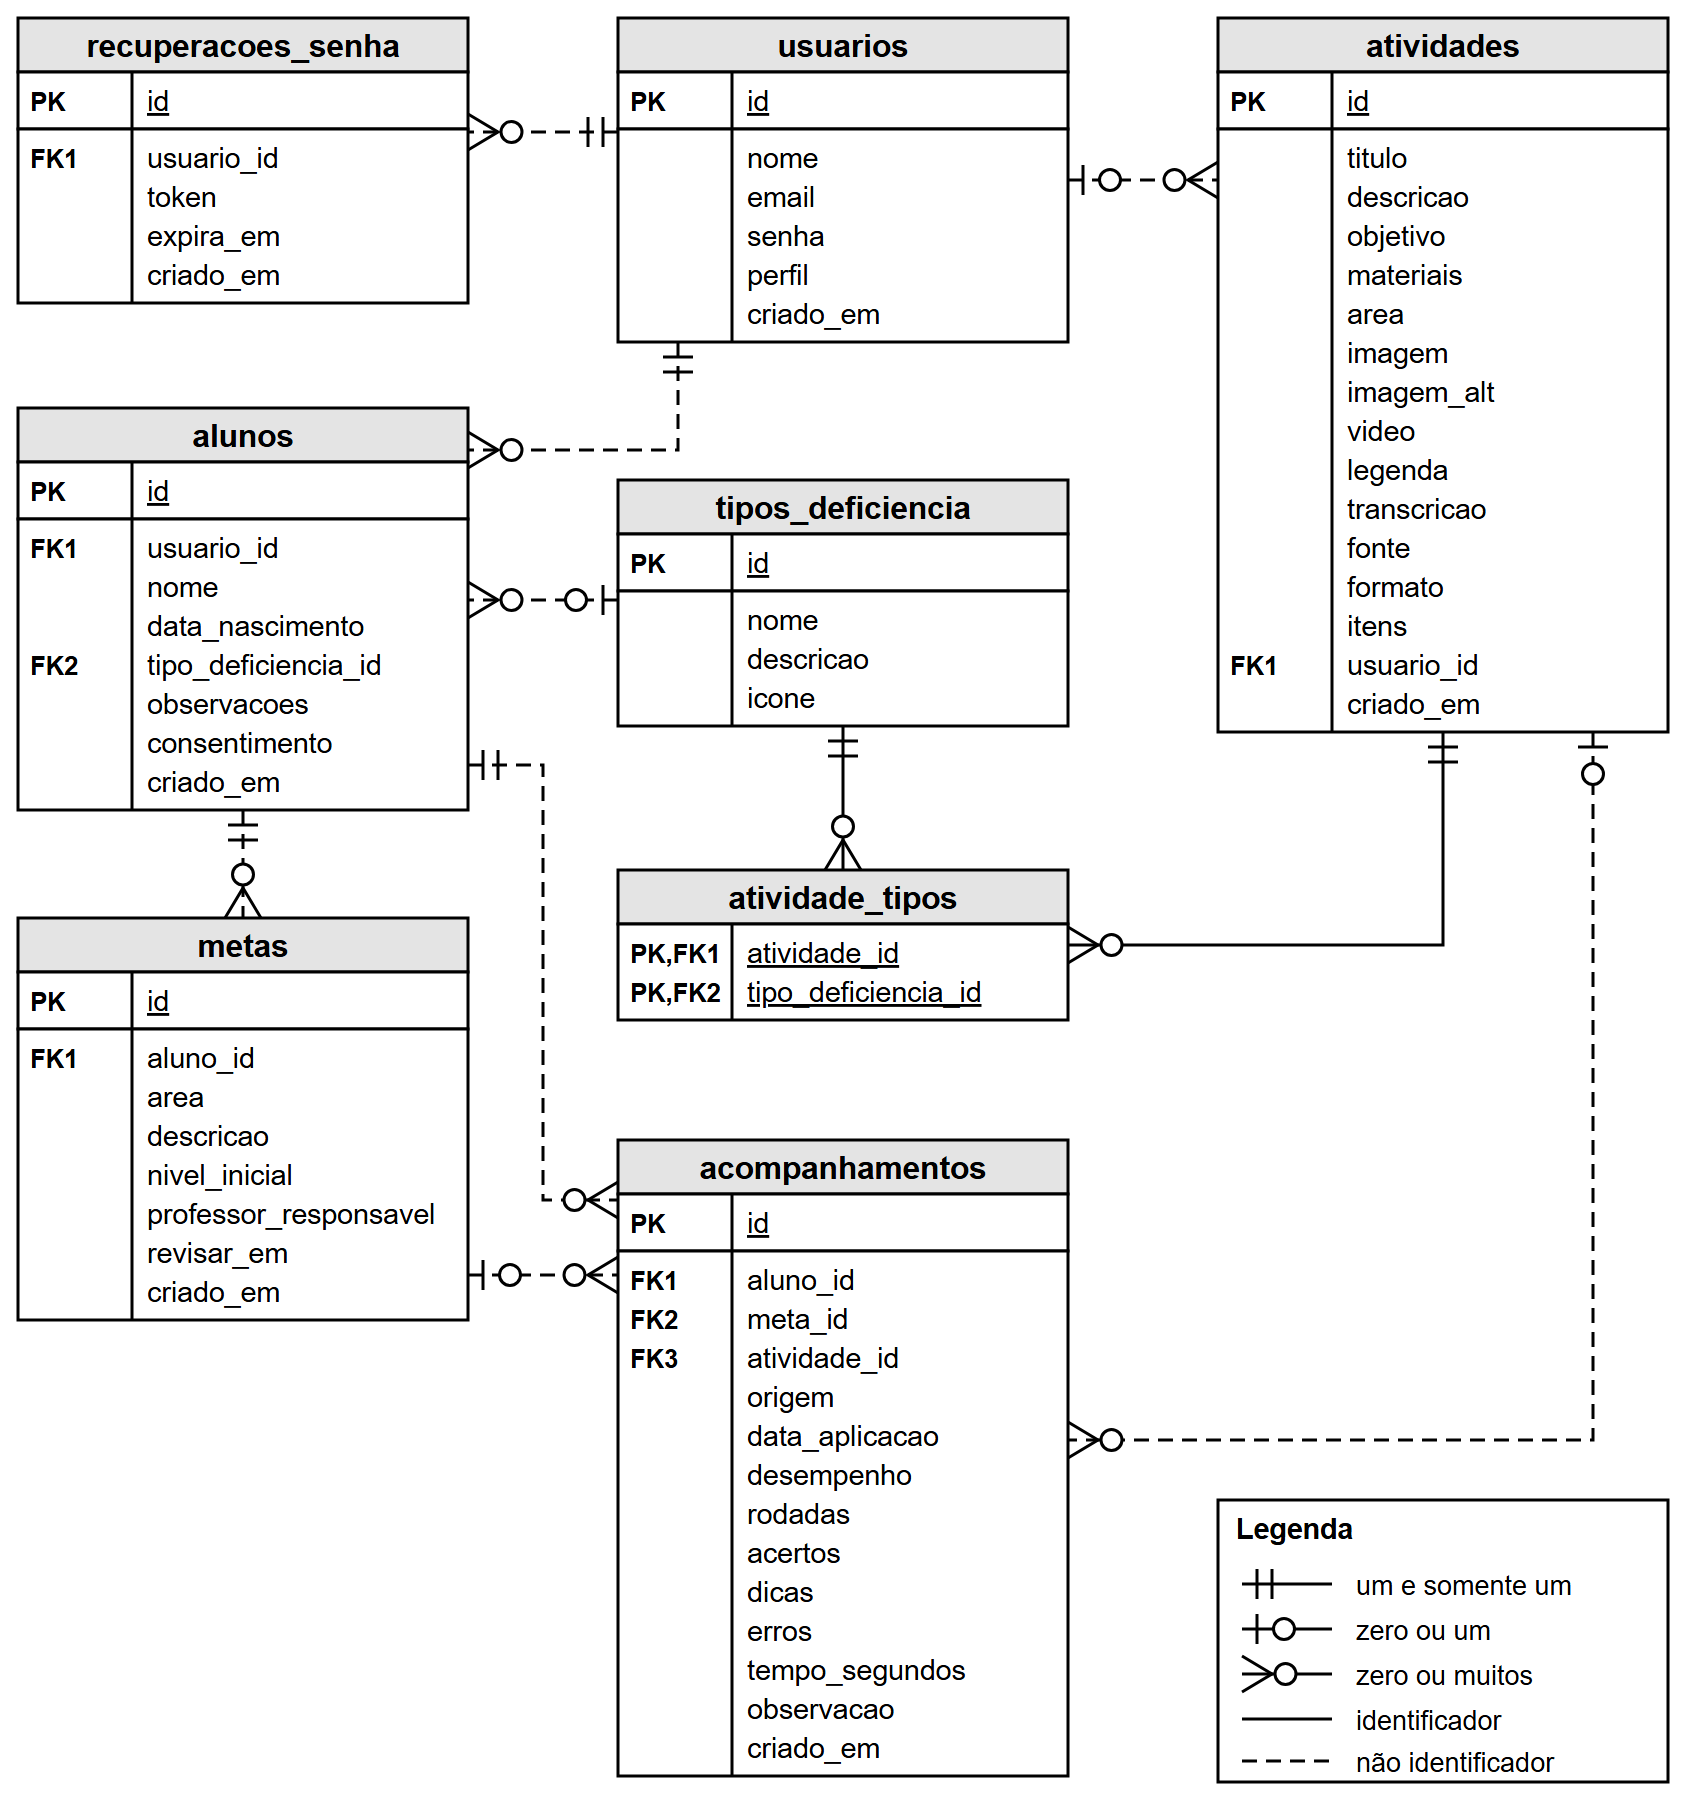
\includegraphics[width=15cm,height=17cm,keepaspectratio]{figuras/figura02-modelo-logico.png}
  \fonte{elaboração própria (2026).}
\end{figure}

O modelo usa a notação pé de galinha, no estilo dos exemplos do Apêndice A de Watt e Eng (2014, p. 129-130). Cada tabela traz o nome no cabeçalho, a chave primária (PK) sublinhada na primeira faixa e as chaves estrangeiras (FK), marcadas como FK1, FK2 e FK3. Os símbolos nas pontas das linhas dão a cardinalidade: dois traços significam um e somente um; um traço e um círculo, zero ou um; o pé de galinha com um círculo, zero ou muitos. Assim, um usuário tem zero ou muitos alunos, e cada aluno pertence a exatamente um usuário; já uma atividade pode não ter usuário, porque \textit{usuario\_id} aceita valor nulo.

A linha contínua marca o relacionamento identificador, em que a chave estrangeira faz parte da chave primária da tabela dependente (WATT; ENG, 2014, p. 41), caso das duas ligações de \textit{atividade\_tipos}; a linha tracejada marca os demais. As tabelas estão dispostas pelas ligações: \textit{usuarios} fica no alto, entre \textit{recuperacoes\_senha} e \textit{atividades}, e \textit{acompanhamentos} fica embaixo, junto das três tabelas de que depende (\textit{alunos}, \textit{metas} e \textit{atividades}). Os nomes de tabelas e colunas seguem um só padrão, o do script SQL: português, letras minúsculas e palavras separadas por sublinhado.

A tabela \textit{usuarios} guarda professores e administradores, com a senha em hash, e \textit{recuperacoes\_senha} guarda os pedidos de nova senha, com o hash do token enviado por e-mail e o prazo de validade. A tabela \textit{tipos\_deficiencia} começa com sete tipos (motora, intelectual, auditiva, visual, TEA, múltipla e “outra / não sei dizer”) e se liga às atividades por \textit{atividade\_tipos}, numa relação muitos-para-muitos. Em \textit{atividades} ficam a área, o formato do mini game, a fonte, obrigatória, e um campo opcional de configuração em JavaScript Object Notation (JSON), descrito na seção~\ref{sec:4.4}.

As três tabelas centrais do acompanhamento são \textit{alunos}, \textit{metas} e \textit{acompanhamentos}. O aluno pertence a um professor e guarda o estudo de caso e o registro do consentimento do responsável. A meta pertence a um aluno e registra a área, a habilidade priorizada, o nível de suporte inicial, o professor responsável e a data de revisão. Cada linha de \textit{acompanhamentos} é o resultado de uma sessão numa meta: data, nível de desempenho, rodadas, acertos, erros, dicas, tempo em segundos e uma observação com o detalhe por jogo.

As regras de exclusão protegem o histórico. Excluir um aluno apaga suas metas e registros. Excluir uma meta ou uma atividade mantém os registros e apenas desfaz o vínculo. Excluir um tipo de deficiência que ainda tem atividades é bloqueado.

A Figura~\ref{fig:3} mostra as mesmas entidades como classes do domínio, num diagrama de classes da UML. A tabela de ligação \textit{atividade\_tipos} aparece como uma associação de muitos para muitos entre \textit{Atividade} e \textit{TipoDeficiencia}, e \textit{recuperacoes\_senha}, que só serve ao controle de acesso, fica de fora.

\begin{figure}[hbp]
  \legendafig{figure}{Diagrama de classes do domínio}{fig:3}
  % Diagrama de classes da UML com Usuario, Aluno, Meta, Acompanhamento, Atividade e TipoDeficiencia, suas associações e as enumerações Perfil, Area, NivelSuporte, Origem e FormatoJogo
  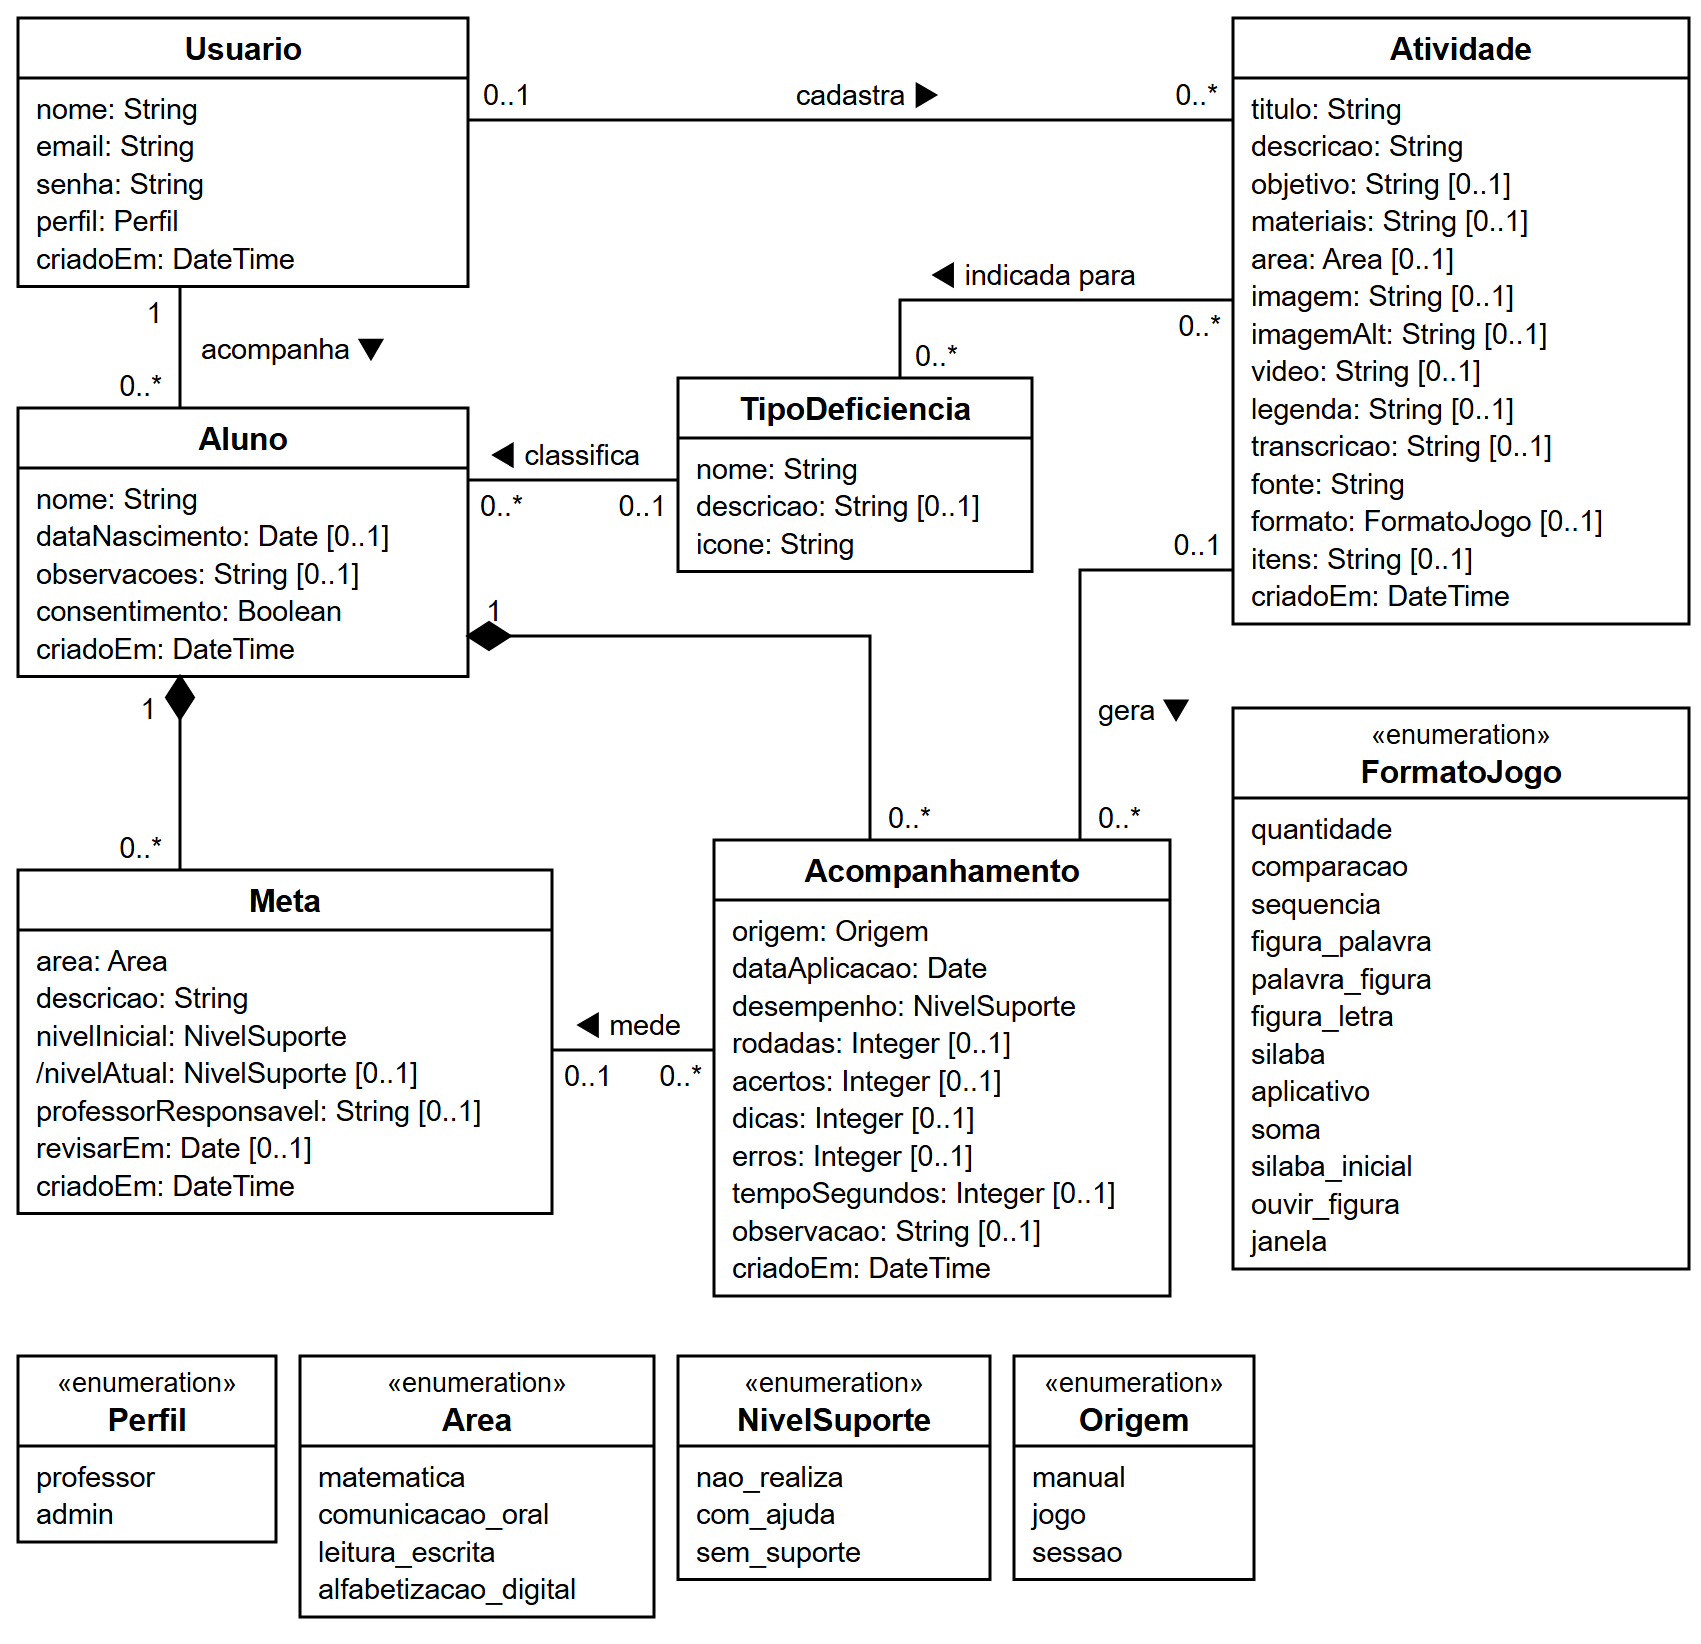
\includegraphics[width=15cm,height=17cm,keepaspectratio]{figuras/figura03-classes.png}
  \fonte{elaboração própria (2026).}
\end{figure}

Na notação da UML (OBJECT MANAGEMENT GROUP, 2017, p. 113, 168, 201 e 202), cada classe tem o nome no primeiro compartimento e os atributos no segundo, na forma nome: Tipo. A multiplicidade [0..1] indica atributo opcional, e a barra antes de \textit{nivelAtual} indica atributo derivado: o nível atual da meta é calculado a partir do registro mais recente. As associações são linhas contínuas com a multiplicidade em cada ponta, e o triângulo junto ao nome dá o sentido da leitura, como em “\textit{Usuario} cadastra \textit{Atividade}”. O losango preto marca a composição: metas e acompanhamentos pertencem a um único aluno e, no sistema, são apagados junto com ele. As cinco enumerações, marcadas com «enumeration», listam os valores aceitos pelos atributos de perfil, área, nível de suporte, origem e formato do jogo; em \textit{Origem}, os valores \textit{manual} e \textit{jogo} só existem por compatibilidade com bancos de versões anteriores, e o sistema atual grava apenas \textit{sessao}. As operações foram omitidas, porque o diagrama descreve os dados do domínio.

\section{Mini games e sessão de atividades}\label{sec:4.4}

Cada atividade do catálogo pertence a uma das quatro áreas e usa um dos 12 formatos de mini game. As rodadas são sorteadas a partir de um catálogo de 14 figuras desenhadas em SVG pelo próprio sistema (bola, bolo, carro, casa, copo, estrela, flor, gato, livro, lua, maçã, pato, peixe e sol), sem arquivos de imagem nem acesso à internet. Cada figura guarda a palavra, a letra inicial e a divisão em sílabas, como ES-TRE-LA, e tem silhueta própria, para que nenhuma informação dependa de cor. O Quadro~\ref{qua:6} descreve os formatos e indica as habilidades da Base Nacional Comum Curricular (BNCC) que cada um exercita.

\begin{tabelaIFTO}
\setlength{\largtab}{\dimexpr\linewidth-8\tabcolsep-5\arrayrulewidth-1pt\relax}
\begin{longtable}{|L{0.1895}|L{0.3499}|L{0.2508}|L{0.2099}|}
\legendatab{quadro}{Formatos de mini game}{qua:6}{4}\\
\hline
\textbf{Formato} & \textbf{O que aparece na tela} & \textbf{Área} & \textbf{BNCC (1º ano)} \\
\hline
\endfirsthead
\multicolumn{4}{@{}r@{}}{\textit{(continuação)}}\\
\hline
\textbf{Formato} & \textbf{O que aparece na tela} & \textbf{Área} & \textbf{BNCC (1º ano)} \\
\hline
\endhead
\multicolumn{4}{@{}r@{}}{\textit{(continua)}}\\
\endfoot
\fontetab{4}{elaboração própria (2026), com as habilidades de Brasil (2018b).}
\endlastfoot
Contar & Figuras repetidas para contar; o aluno escolhe entre todos os numerais, de 1 ao maior número da atividade & Alfabetização Matemática & EF01MA01, EF01MA02 \\ \hline
Comparar & Dois grupos de figuras; o aluno escolhe o que tem mais, ou menos & Alfabetização Matemática & EF01MA03 \\ \hline
Sequência & Sequência de numerais com uma lacuna e três numerais para completá-la & Alfabetização Matemática & EF01MA10 \\ \hline
Juntar & Dois grupos de figuras iguais; o aluno escolhe o total entre três numerais & Alfabetização Matemática & EF01MA06, EF01MA08 \\ \hline
Figura e palavra & Uma figura e três palavras & Leitura e Escrita & EF12LP01 \\ \hline
Palavra e figura & Uma palavra escrita e três figuras & Leitura e Escrita & EF12LP01 \\ \hline
Letra inicial & Uma figura e três letras & Leitura e Escrita & EF01LP07 \\ \hline
Sílaba inicial & Uma figura e três sílabas & Leitura e Escrita & EF01LP08, EF01LP09 \\ \hline
Sílaba que falta & A figura e o nome com uma sílaba faltando; três sílabas para completar & Leitura e Escrita & EF01LP08, EF01LP13 \\ \hline
Ouvir e escolher & Botão “Ouvir a palavra”, que usa a voz do navegador sem mostrar a palavra escrita, e três figuras & Comunicação Oral & Competência geral 4 \\ \hline
Abrir, usar e fechar & Tablet simulado: abrir o aplicativo pedido entre quatro ícones, usar o jogo de palavras dentro dele em três rodadas e fechá-lo & Alfabetização Digital & Competência geral 5 \\ \hline
Botões da janela & Aplicativo aberto; o aluno toca no botão pedido: Fechar, Minimizar ou Voltar & Alfabetização Digital & Competência geral 5 \\ \hline
\end{longtable}
\end{tabelaIFTO}

A última coluna liga cada formato às habilidades do 1º ano da BNCC. Em Matemática, os jogos trabalham o número como indicador de quantidade e a contagem (EF01MA01 e EF01MA02), a comparação de quantidades para indicar “tem mais” ou “tem menos” (EF01MA03), os fatos básicos da adição e o significado de juntar, com o suporte de imagens (EF01MA06 e EF01MA08), e os elementos ausentes em sequências de números naturais (EF01MA10) (BRASIL, 2018b, p. 279). Em Língua Portuguesa, trabalham a leitura de palavras (EF12LP01), a relação entre fonemas e letras (EF01LP07) e a relação entre sílabas e sua escrita, comparando sílabas iniciais, mediais e finais (EF01LP08, EF01LP09 e EF01LP13) (BRASIL, 2018b, p. 99, 101). Os jogos de Comunicação Oral não têm habilidade específica do 1º ano e se ligam à competência geral 4, que trata do uso de diferentes linguagens, entre elas a oral; os de Alfabetização Digital se ligam à competência geral 5, que trata de compreender e utilizar tecnologias digitais (BRASIL, 2018b, p. 9). A correspondência é parcial: cada mini game exercita uma parte da habilidade, em formato de múltipla escolha, e não substitui o trabalho do professor com ela.

Um campo opcional de configuração, gravado em JSON na atividade, permite que um mesmo formato gere atividades diferentes. A chave \textit{figuras} restringe as figuras sorteadas, por exemplo a palavras parecidas como bola, bolo, gato e pato; a chave \textit{app} escolhe o aplicativo do tablet simulado; e a chave \textit{maximo}, de 2 a 10, define o maior número dos jogos de matemática. É assim que existem, por exemplo, “Contar e escolher o numeral (até 5)” e “(até 10)”.

O catálogo inicial tem 24 atividades, seis por área, listadas no Quadro~\ref{qua:7}. Seis atividades por área permitem variar o exercício e a dificuldade dentro de uma mesma meta. Todas foram propostas neste projeto e ainda não passaram por validação de profissionais da educação especial.

\begin{tabelacurta}
\setlength{\largtab}{\dimexpr\linewidth-4\tabcolsep-3\arrayrulewidth-1pt\relax}
\legenda{quadro}{Atividades iniciais do catálogo, por área}\label{qua:7}\vspace{4pt}
\begin{tabular}{|L{0.3571}|L{0.6429}|}
\hline
\textbf{Área} & \textbf{Atividades} \\
\hline
Alfabetização Matemática & Contar e escolher o numeral (até 5); Contar e escolher o numeral (até 10); Comparar quantidades: mais e menos (até 5); Comparar quantidades: mais e menos (até 10); Completar a sequência de numerais (até 10); Juntar quantidades (até 5) \\ \hline
Leitura e Escrita & Associar figura e palavra; Associar figura e palavra: palavras parecidas; Ler a palavra e escolher a figura; Identificar a letra inicial da figura; Identificar a sílaba inicial da figura; Completar a sílaba que falta \\ \hline
Comunicação Oral & Ouvir a palavra e escolher a figura; Ouvir e escolher: animais; Ouvir e escolher: céu e natureza; Ouvir e escolher: objetos; Ouvir e escolher: coisas da mesa; Ouvir e escolher: palavras parecidas \\ \hline
Alfabetização Digital & Abrir, usar e fechar: Palavras e figuras; Abrir, usar e fechar: Calendário; Abrir, usar e fechar: Relógio; Abrir, usar e fechar: Fotos; Abrir, usar e fechar: Música; Botões da janela: fechar, minimizar e voltar \\ \hline
\end{tabular}
\fonte{elaboração própria (2026).}
\end{tabelacurta}

As atividades estão ligadas a todos os tipos de deficiência, com duas exceções. Nenhuma está ligada à deficiência visual, porque todas dependem de ver as figuras, e as de ouvir a palavra não estão ligadas à deficiência auditiva. Essa ligação é usada nas sugestões de atividades para cada meta.

A sessão de atividades é o caminho em que o aluno responde e o resultado é medido sem digitação do professor. A Figura~\ref{fig:4} mostra, num diagrama de sequência da UML, a troca de mensagens entre os participantes de uma sessão.

\begin{figure}[hbp]
  \legendafig{figure}{Diagrama de sequência da sessão de mini games}{fig:4}
  % Diagrama de sequência da UML com Professor, Aluno, SessaoController, SessaoAtividade e Acompanhamento e os fragmentos loop, opt e alt
  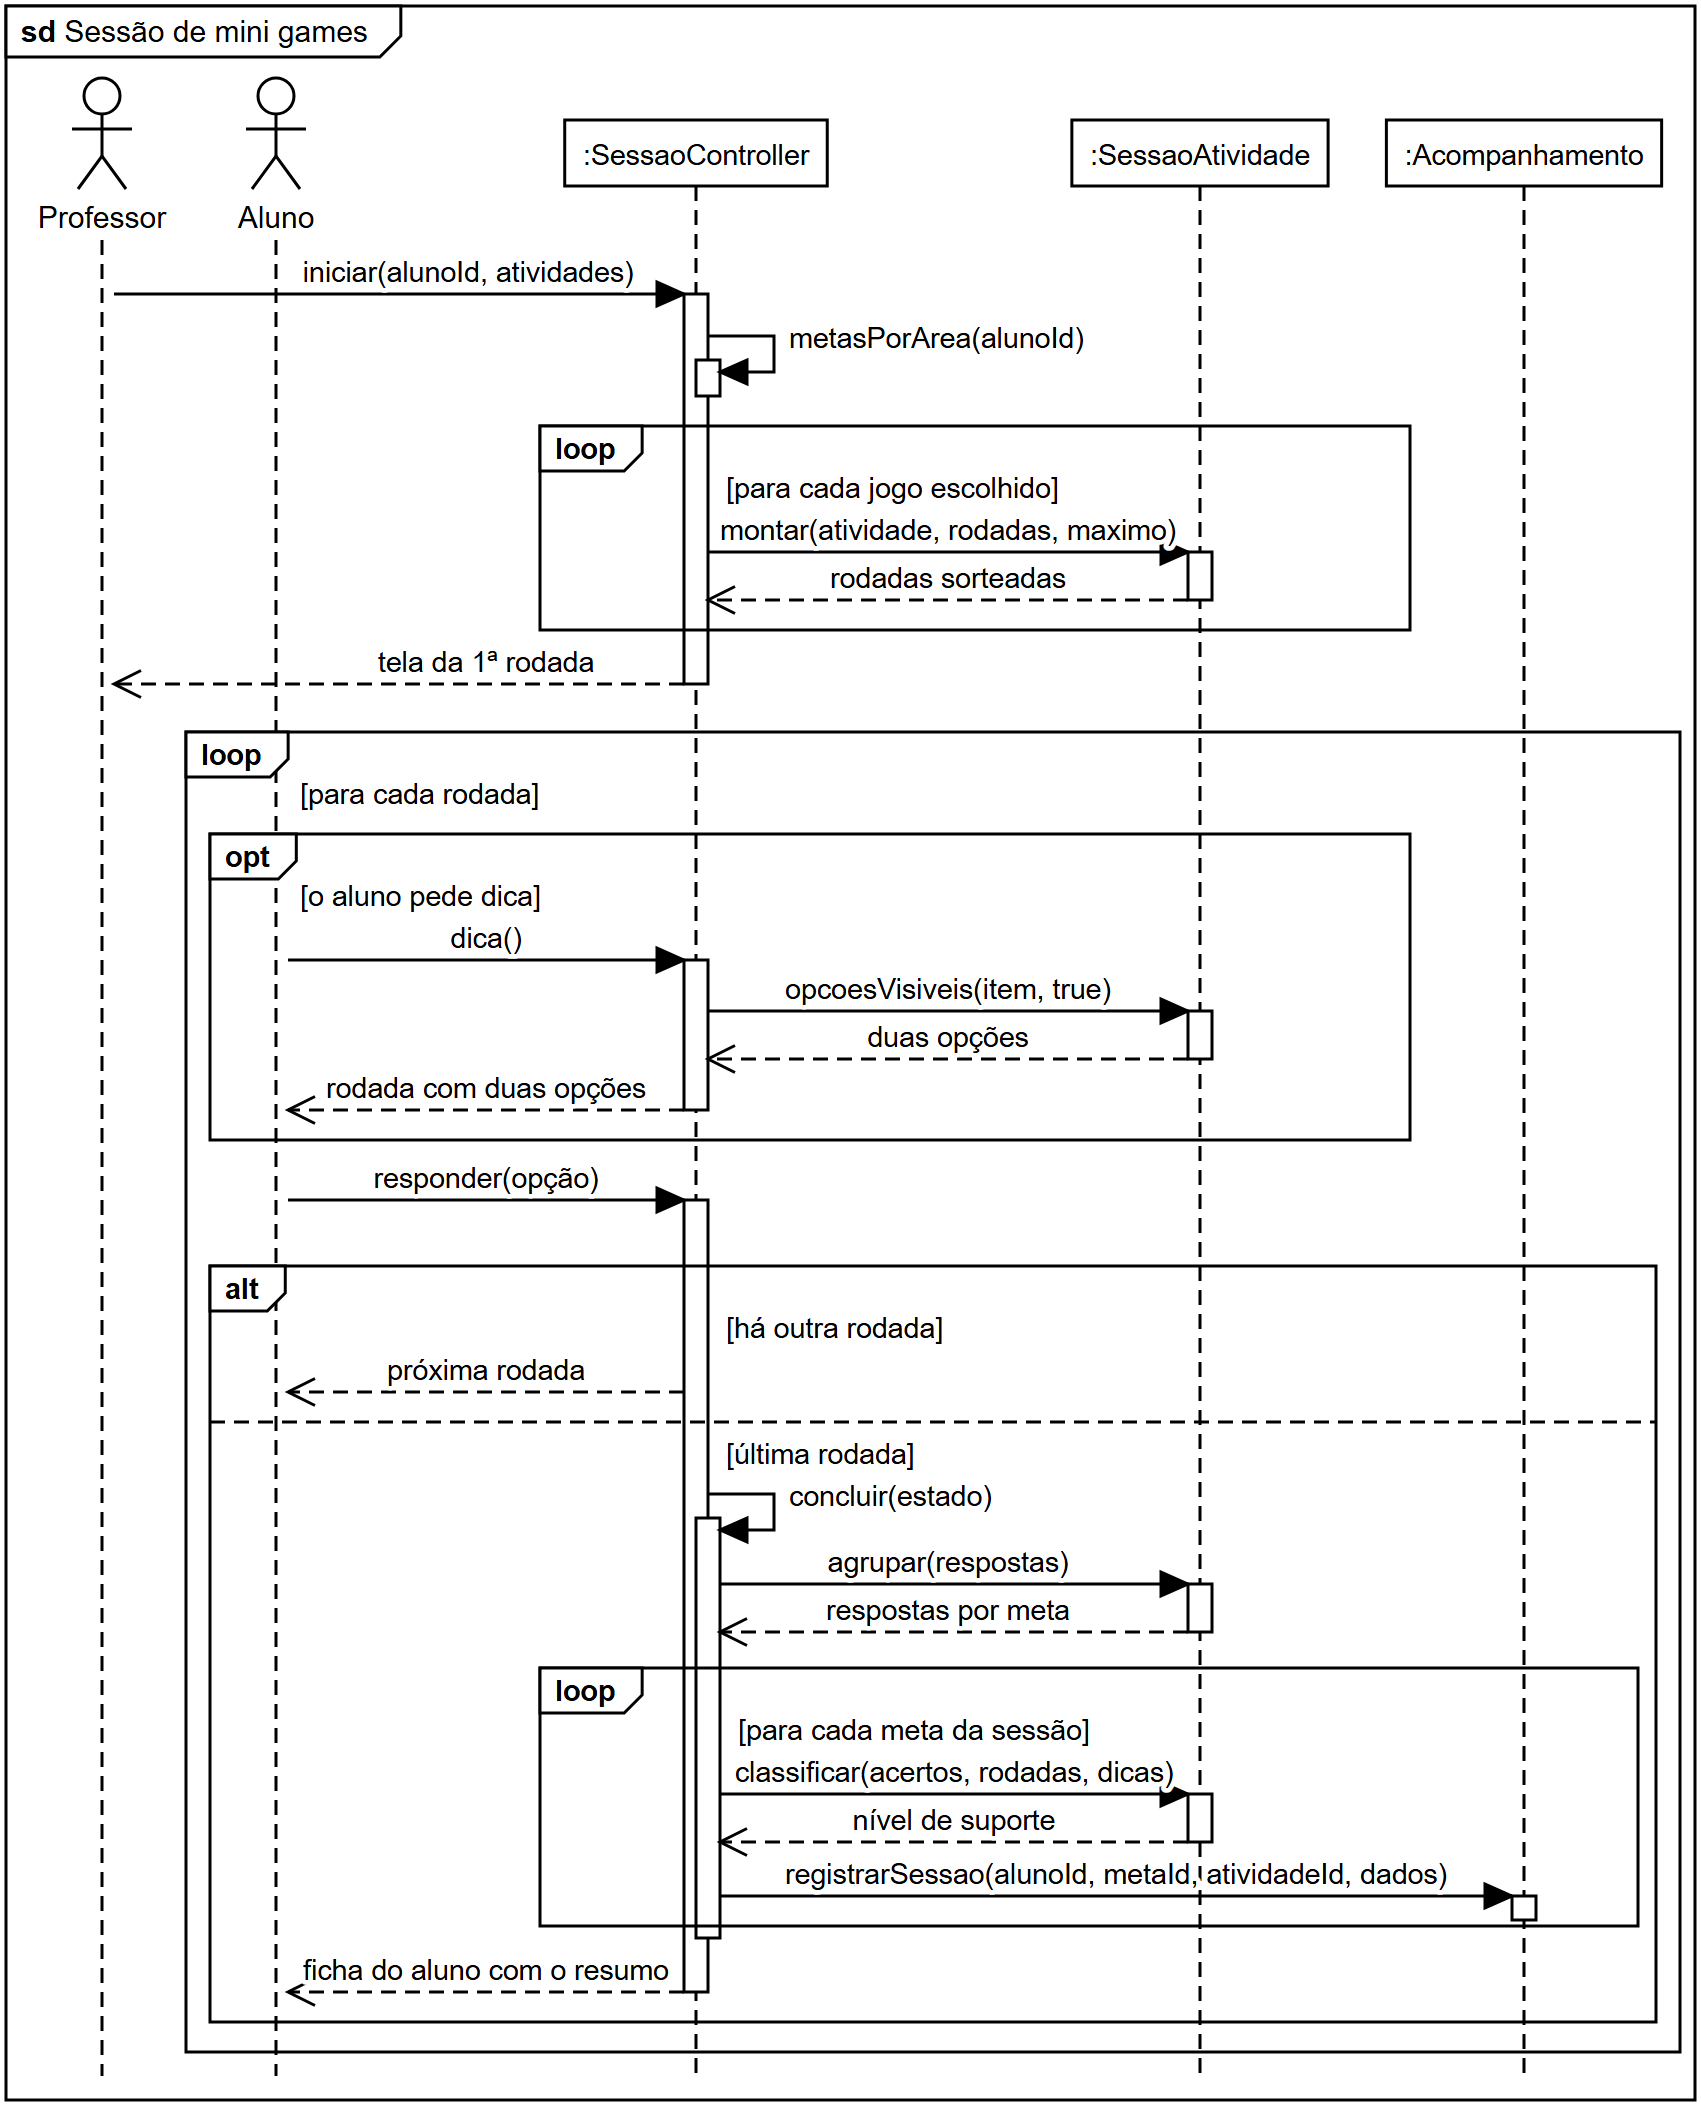
\includegraphics[width=15cm,height=17cm,keepaspectratio]{figuras/figura04-sequencia.png}
  \fonte{elaboração própria (2026).}
\end{figure}

Na Figura~\ref{fig:4}, cada participante tem uma linha de vida tracejada: o professor e o aluno, como atores, e três objetos do sistema, o controlador da sessão (\textit{SessaoController}), o serviço que monta e classifica as rodadas (\textit{SessaoAtividade}) e o modelo que grava os registros (\textit{Acompanhamento}). O banco de dados não aparece, porque não é um objeto da aplicação: a gravação é feita dentro do modelo. A moldura com o rótulo sd delimita a interação; as setas de ponta cheia são chamadas, as tracejadas são retornos, e os retângulos estreitos sobre as linhas de vida mostram quando cada objeto está em execução (OBJECT MANAGEMENT GROUP, 2017, p. 568 e 577). A seta que volta para o próprio controlador, como em \textit{metasPorArea(alunoId)}, é uma chamada a si mesmo; essa, logo no início, escolhe a meta em que cada área será registrada.

Os retângulos com um nome no canto superior esquerdo são fragmentos combinados. O operador do canto diz o que acontece com as mensagens de dentro, e a condição entre colchetes, chamada guarda, diz quando acontece; a guarda fica junto à linha de vida do primeiro evento do fragmento (OBJECT MANAGEMENT GROUP, 2017, p. 583-585). A Figura~\ref{fig:4} tem cinco fragmentos, de três tipos:

\begin{alineasIFTO}
  \item loop [para cada jogo escolhido], no início da Figura~\ref{fig:4}: repete a chamada \textit{montar(atividade, rodadas, maximo)} uma vez para cada jogo marcado pelo professor; cada repetição devolve as cinco rodadas sorteadas daquele jogo, e as rodadas de todos os jogos formam a sessão;
  \item loop [para cada rodada], que ocupa a maior parte da Figura~\ref{fig:4}: repete, rodada a rodada, a troca entre o aluno e o sistema, com o pedido opcional de dica, a resposta e a conferência; o laço termina na última rodada;
  \item opt [o aluno pede dica], dentro do loop das rodadas: o trecho só acontece quando o aluno toca em “Pedir dica”; então o controlador pede ao serviço as opções da rodada com a dica, \textit{opcoesVisiveis(item, true)}, e a rodada volta com duas opções; sem o pedido, nada do que está dentro do opt acontece, e a rodada segue com todas as opções;
  \item alt [há outra rodada] e [última rodada], logo depois da conferência da resposta: executa um dos dois trechos separados pela linha tracejada; se há outra rodada, o aluno recebe a próxima; na última, o controlador executa \textit{concluir(estado)}, pede ao serviço que agrupe as respostas por meta e devolve a ficha do aluno com o resumo;
  \item loop [para cada meta da sessão], dentro do segundo trecho do alt: para cada meta que teve jogos na sessão, classifica o nível de suporte com \textit{classificar(acertos, rodadas, dicas)} e grava um registro com \textit{registrarSessao(alunoId, metaId, atividadeId, dados)}.
\end{alineasIFTO}

O professor inicia a sessão e entrega o aparelho ao aluno; por isso a primeira rodada volta ao professor, e a ficha, resposta à última rodada, aparece no mesmo aparelho. O botão Cancelar, que encerra a sessão sem gravar, não foi representado.

A sessão segue seis passos:

\begin{passos}
  \item Na ficha do aluno, o professor marca um ou mais jogos, ou usa o botão “Fazer na tela” de uma sugestão, que já indica a meta. Sem indicação, cada jogo vai para a primeira meta do aluno na mesma área, mostrada ao lado do jogo; os jogos de áreas sem meta ficam desabilitados.
  \item O sistema sorteia cinco rodadas por jogo. No formato de aplicativo, as cinco rodadas são as etapas: abrir, três rodadas de uso e fechar.
  \item A tela mostra uma rodada por vez, com o enunciado, uma cena desenhada e botões grandes; um toque já responde. Essa tela não traz o menu do professor, para que a criança não saia do jogo por engano; só o botão Cancelar, que pede confirmação, encerra a sessão antes do fim.
  \item O aluno pode pedir uma dica por rodada. Nas rodadas com três ou mais opções, a dica deixa apenas duas, a correta e uma errada, numa ordem que não revela qual é a certa. No jogo de comparar, que já tem só duas opções, a dica não é oferecida.
  \item Cada resposta é conferida no servidor e guardada com o acerto, o uso de dica e os segundos passados desde a resposta anterior.
  \item Ao final, as respostas são somadas por meta, cada meta recebe um nível de suporte e um registro é gravado para cada meta, com o detalhe por jogo. Cancelar a sessão encerra tudo sem gravar.
\end{passos}

No formato de aplicativo, as três etapas são registradas à parte, e o tempo até o aluno abrir o aplicativo aparece no detalhe do registro.

\section{Classificação e indicadores de evolução}\label{sec:4.5}

Ao fim da sessão, o resultado de cada meta é classificado em um dos três níveis do AppPEI pela regra do Quadro~\ref{qua:8}.

\begin{tabelacurta}
\setlength{\largtab}{\dimexpr\linewidth-4\tabcolsep-3\arrayrulewidth-1pt\relax}
\legenda{quadro}{Regra de classificação do nível de suporte}\label{qua:8}\vspace{4pt}
\begin{tabular}{|L{0.5924}|L{0.4076}|}
\hline
\textbf{Resultado da sessão na meta} & \textbf{Nível registrado} \\
\hline
Nenhum acerto & Não realiza \\ \hline
Todas as rodadas certas, sem nenhuma dica & Realiza sem necessidade de suporte \\ \hline
Qualquer outro caso: acertos parciais, ou todos certos com dica & Realiza com ajuda \\ \hline
\end{tabular}
\fonte{elaboração própria (2026), com os níveis de Francisco (2023).}
\end{tabelacurta}

A regra exige a evidência mais forte para o nível mais alto: acertar tudo sem nenhum apoio. Ela é uma hipótese do protótipo (seção~\ref{sec:5.4}). Um ponto a discutir com professores é que o nível “realiza com ajuda” reúne duas situações diferentes: o aluno que usou dica e o aluno que não usou dica, mas errou alguma rodada.

Com as sessões de uma meta em ordem cronológica, o sistema calcula quatro indicadores:

\begin{alineasIFTO}
  \item acerto médio: total de acertos dividido pelo total de rodadas, em porcentagem;
  \item autonomia: porcentagem de sessões classificadas como “realiza sem necessidade de suporte”;
  \item sessões com dica: porcentagem de sessões em que houve pelo menos uma dica;
  \item variação: diferença, em pontos percentuais, entre o acerto médio da segunda e o da primeira metade das sessões, a partir de seis sessões.
\end{alineasIFTO}

Sendo $t_i$ a taxa de acerto da sessão $i$ ($\mathit{acertos} \div \mathit{rodadas} \times 100$), $n$ o número de sessões e $m$ a metade de $n$ arredondada para baixo, a variação é:

\begin{equation}
\Delta = \frac{1}{m}\sum_{i=n-m+1}^{n} t_i \;-\; \frac{1}{m}\sum_{i=1}^{m} t_i, \qquad m = \left\lfloor \frac{n}{2} \right\rfloor, \quad n \geq 6
\label{eq:variacao}
\end{equation}

Quando $n$ é ímpar, a sessão do meio fica fora das duas médias. O mínimo de seis sessões evita que cada metade tenha uma ou duas sessões, caso em que um único dia atípico mudaria o resultado. A Tabela~\ref{tab:1} mostra um exemplo com dados fictícios.

\begin{tabelacurta}
\setlength{\largtab}{\dimexpr\linewidth-10\tabcolsep-0\arrayrulewidth-1pt\relax}
\legenda{table}{Exemplo fictício de seis sessões de uma meta}\label{tab:1}\vspace{4pt}
\begin{tabular}{C{0.0982}C{0.2223}C{0.0858}C{0.1603}L{0.4334}}
\hline
\textbf{Sessão} & \textbf{Acertos (de 5)} & \textbf{Dicas} & \textbf{Acerto (\%)} & \textbf{Nível registrado} \\
\hline
1 & 2 & 2 & 40,0 & Realiza com ajuda \\
2 & 2 & 1 & 40,0 & Realiza com ajuda \\
3 & 3 & 1 & 60,0 & Realiza com ajuda \\
4 & 4 & 1 & 80,0 & Realiza com ajuda \\
5 & 4 & 0 & 80,0 & Realiza com ajuda \\
6 & 5 & 0 & 100,0 & Realiza sem necessidade de suporte \\
\hline
\end{tabular}
\fonte{elaboração própria (2026), com dados fictícios.}
\end{tabelacurta}

No exemplo, o acerto médio é 66,7\% (20 acertos em 30 rodadas), a autonomia é 16,7\% (uma sessão em seis) e as sessões com dica são 66,7\% (quatro em seis). A média da primeira metade é 46,7\% e a da segunda, 86,7\%, o que dá uma variação de +40,0 pontos percentuais. A sessão 5 mostra a nuance da regra: sem dica, mas com um erro, ela ainda é registrada como “realiza com ajuda”.

\section{Gráficos de evolução}\label{sec:4.6}

Na ficha do aluno, a seção “Evolução nas sessões na tela” mostra uma tabela com os indicadores de cada meta e, para cada meta com sessões, um cartão com dois gráficos desenhados em SVG pelo servidor, sem biblioteca externa. A Figura~\ref{fig:5} reproduz esse cartão para os dados da Tabela~\ref{tab:1}; ela foi gerada com as mesmas classes que o sistema usa na ficha, alimentadas com os dados fictícios do exemplo.

\begin{figure}[hbp]
  \legendafig{figure}{Gráficos de evolução gerados pelo UNIA para os dados da Tabela 1}{fig:5}
  % Linha do acerto nas seis sessões, de 40% a 100%, com as médias tracejadas de 46,7% e 86,7% e a linha do tempo do nível de suporte
  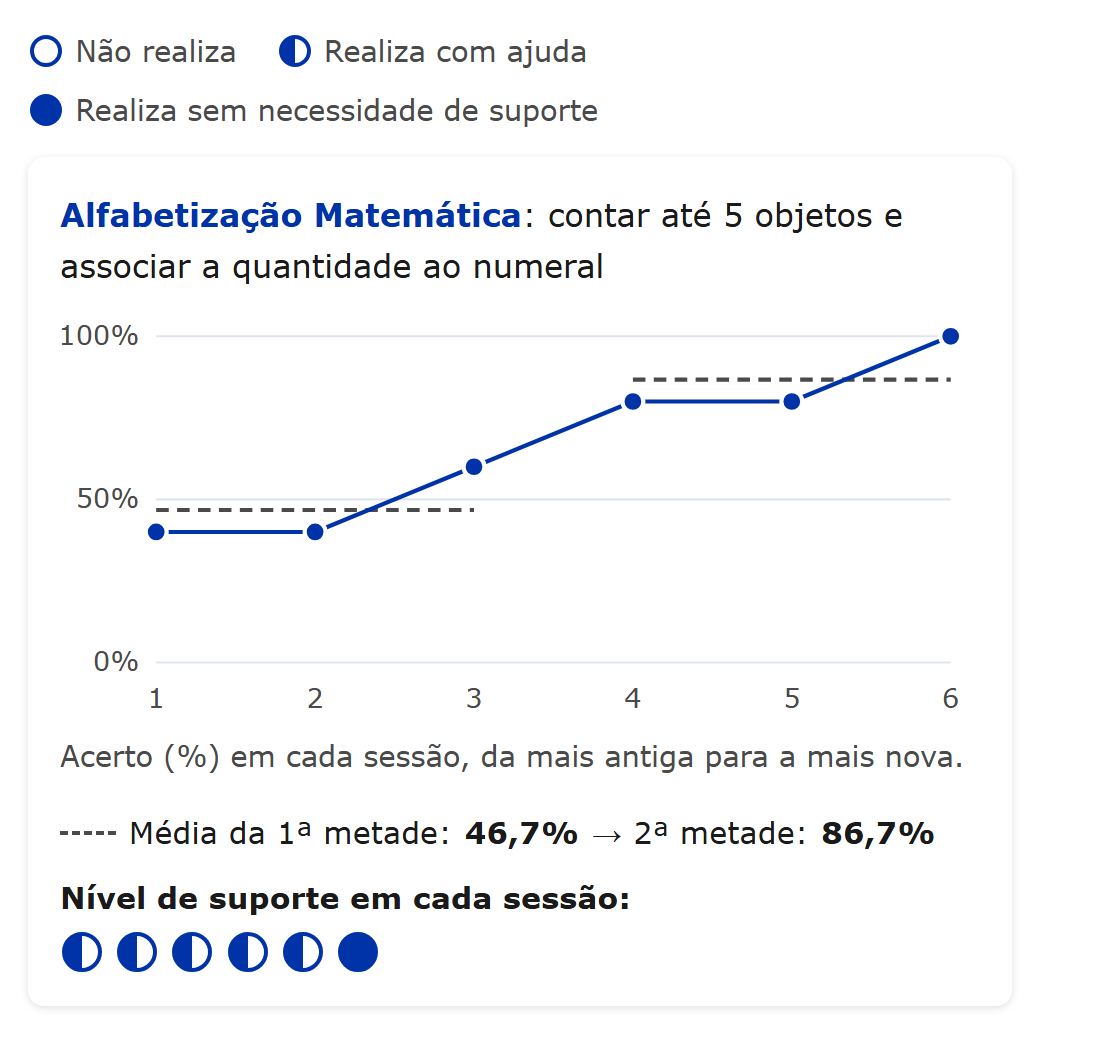
\includegraphics[width=14.5cm,height=17cm,keepaspectratio]{figuras/figura05-graficos-evolucao.png}
  \fonte{elaboração própria (2026), com dados fictícios.}
\end{figure}

O primeiro gráfico é uma linha com a taxa de acerto de cada sessão, da mais antiga para a mais nova. A partir de seis sessões, duas linhas tracejadas mostram a média de cada metade, e a distância vertical entre elas é a variação; os valores das médias aparecem em texto abaixo do gráfico, para não cobrir os pontos. Ao passar o mouse sobre um ponto, o sistema mostra a data, os acertos e as dicas daquela sessão.

O segundo gráfico é uma linha do tempo do nível de suporte, com um símbolo por sessão: círculo vazio para “não realiza”, meio cheio para “realiza com ajuda” e cheio para “realiza sem necessidade de suporte”. Como a forma muda, e não apenas a cor, o nível pode ser lido sem depender da percepção de cores. Cada gráfico tem também uma descrição em texto, lida por leitores de tela, com os valores de todas as sessões e as médias, e os números exatos continuam na tabela da ficha.

\section{Segurança e privacidade}\label{sec:4.7}

O UNIA guarda dados de crianças, e parte deles, como o tipo de deficiência e o estudo de caso, pode ser considerada dado referente à saúde, que a Lei Geral de Proteção de Dados Pessoais (LGPD) classifica como dado pessoal sensível (BRASIL, 2018a, art. 5º, II). A mesma lei exige que o tratamento de dados de crianças atenda ao seu melhor interesse e conte com o consentimento específico de pelo menos um dos pais ou do responsável legal (BRASIL, 2018a, art. 14). Por isso, a segurança foi tratada como requisito desde a versão 2. O Quadro~\ref{qua:9} relaciona as ameaças consideradas, baseadas nas categorias do Top 10 do Open Worldwide Application Security Project (OWASP), lista dos riscos mais críticos de segurança em aplicações web (OWASP FOUNDATION, 2021), aos mecanismos adotados.

\begin{tabelaIFTO}
\setlength{\largtab}{\dimexpr\linewidth-4\tabcolsep-3\arrayrulewidth-1pt\relax}
\begin{longtable}{|L{0.4043}|L{0.5957}|}
\legendatab{quadro}{Ameaças e mecanismos de segurança}{qua:9}{2}\\
\hline
\textbf{Ameaça} & \textbf{Mecanismo no UNIA} \\
\hline
\endfirsthead
\multicolumn{2}{@{}r@{}}{\textit{(continuação)}}\\
\hline
\textbf{Ameaça} & \textbf{Mecanismo no UNIA} \\
\hline
\endhead
\multicolumn{2}{@{}r@{}}{\textit{(continua)}}\\
\endfoot
\fontetab{2}{elaboração própria (2026).}
\endlastfoot
Vazamento de senhas do banco & Senhas guardadas com \textit{password\_hash()} e conferidas com \textit{password\_verify()} \\ \hline
Injeção de SQL & PDO com consultas parametrizadas e emulação de prepared statements desligada \\ \hline
Script injetado na página (XSS) & Escape de toda saída de dado digitado pelo usuário \\ \hline
Formulário forjado (CSRF) & Token por sessão, conferido pelo roteador em todo POST \\ \hline
Acesso sem login ou sem o perfil exigido & Verificações de acesso nas rotas: visitante, logado ou administrador \\ \hline
Acesso a dados de outro professor & Consultas filtradas pelo professor logado; resposta 404 para dados de terceiros \\ \hline
Força bruta no login & Bloqueio de 5 minutos após 5 tentativas erradas, contadas por sessão \\ \hline
Sequestro de sessão & Cookie \textit{HttpOnly} e \textit{SameSite}; novo identificador de sessão no login \\ \hline
Roubo do token de recuperação de senha & Só o hash Secure Hash Algorithm de 256 bits (SHA-256) do token é gravado; uso único; validade de 60 minutos \\ \hline
Envio de arquivo malicioso & Conferência do tipo real do arquivo, limite de 2 MB, nome aleatório e pasta sem execução de PHP \\ \hline
Exposição de arquivos internos e de erros & Apenas a pasta \textit{public} é servida; os erros vão para o log, e a tela mostra mensagem genérica \\ \hline
\end{longtable}
\end{tabelaIFTO}

Na privacidade, além do isolamento entre professores do Quadro~\ref{qua:9}, o cadastro do aluno só é aceito quando o professor confirma ter a autorização do responsável para registrar os dados, e o formulário de atividades orienta a não enviar fotos de crianças sem autorização. A falta de criptografia das observações do estudo de caso está entre as limitações da seção~\ref{sec:5.4}.

\section{Acessibilidade}\label{sec:4.8}

As telas seguem práticas inspiradas na WCAG 2.1 (W3C, 2018): idioma da página definido como português; rótulos em todos os campos; link para pular direto ao conteúdo; foco visível na navegação por teclado; resumo de erros anunciado aos leitores de tela, com link para cada campo; tabelas com legenda e cabeçalhos associados; texto alternativo obrigatório nas imagens das atividades; campos para legenda e transcrição dos vídeos; e respeito à preferência do usuário por menos animação.

Nos mini games, os botões têm pelo menos 44 por 44 pixels, o tamanho mínimo de alvo de toque do critério 2.5.5 da WCAG 2.1 (W3C, 2018), e um toque já responde. Nenhuma informação depende só de cor, como descrito nas seções~\ref{sec:4.4} e~\ref{sec:4.6}. O mini game de ouvir a palavra usa a síntese de fala da Web Speech API, que lê um texto em voz alta com o sintetizador do dispositivo (MOZILLA, 2026); por isso, a voz em português depende do navegador e do sistema.

Há uma escolha com custo. Nas rodadas, as figuras são tratadas como decorativas para os leitores de tela, e os botões recebem rótulos neutros, como “Figura~\ref{fig:1}”, porque dizer o nome da figura entregaria a resposta. Com isso, os mini games não atendem alunos com deficiência visual, limitação discutida na seção~\ref{sec:5.4}.

Como não houve auditoria de acessibilidade (seção~\ref{sec:5.4}), este trabalho afirma que o UNIA segue práticas inspiradas na WCAG 2.1, e não que atende às diretrizes.

\section{Telas do sistema}\label{sec:4.9}

As Figuras~\ref{fig:6} a~\ref{fig:8} mostram telas do UNIA com dados fictícios. A ficha do aluno (Figura~\ref{fig:6}) reúne numa só página o estudo de caso, as metas com o nível atual, a tabela e os gráficos de evolução, as sugestões de atividades, o formulário da sessão e o histórico; a figura mostra o trecho das metas e da evolução. Na rodada (Figura~\ref{fig:7}), a tela mostra o enunciado, a cena desenhada e um botão grande para cada numeral; abaixo dos botões, fora do recorte, ficam “Pedir dica” e “Cancelar”. No formulário da sessão (Figura~\ref{fig:8}), cada jogo indica a meta em que o resultado será gravado, e os jogos de áreas sem meta aparecem desabilitados. O catálogo de atividades, que não aparece nas figuras, permite buscar atividades e filtrá-las por área e por tipo de deficiência.

\begin{figure}[hbp]
  \legendafig{figure}{Ficha do aluno, com metas, indicadores e gráficos}{fig:6}
  % Ficha do aluno com a tabela de metas, os indicadores de evolução e o início do gráfico de uma meta de leitura e escrita
  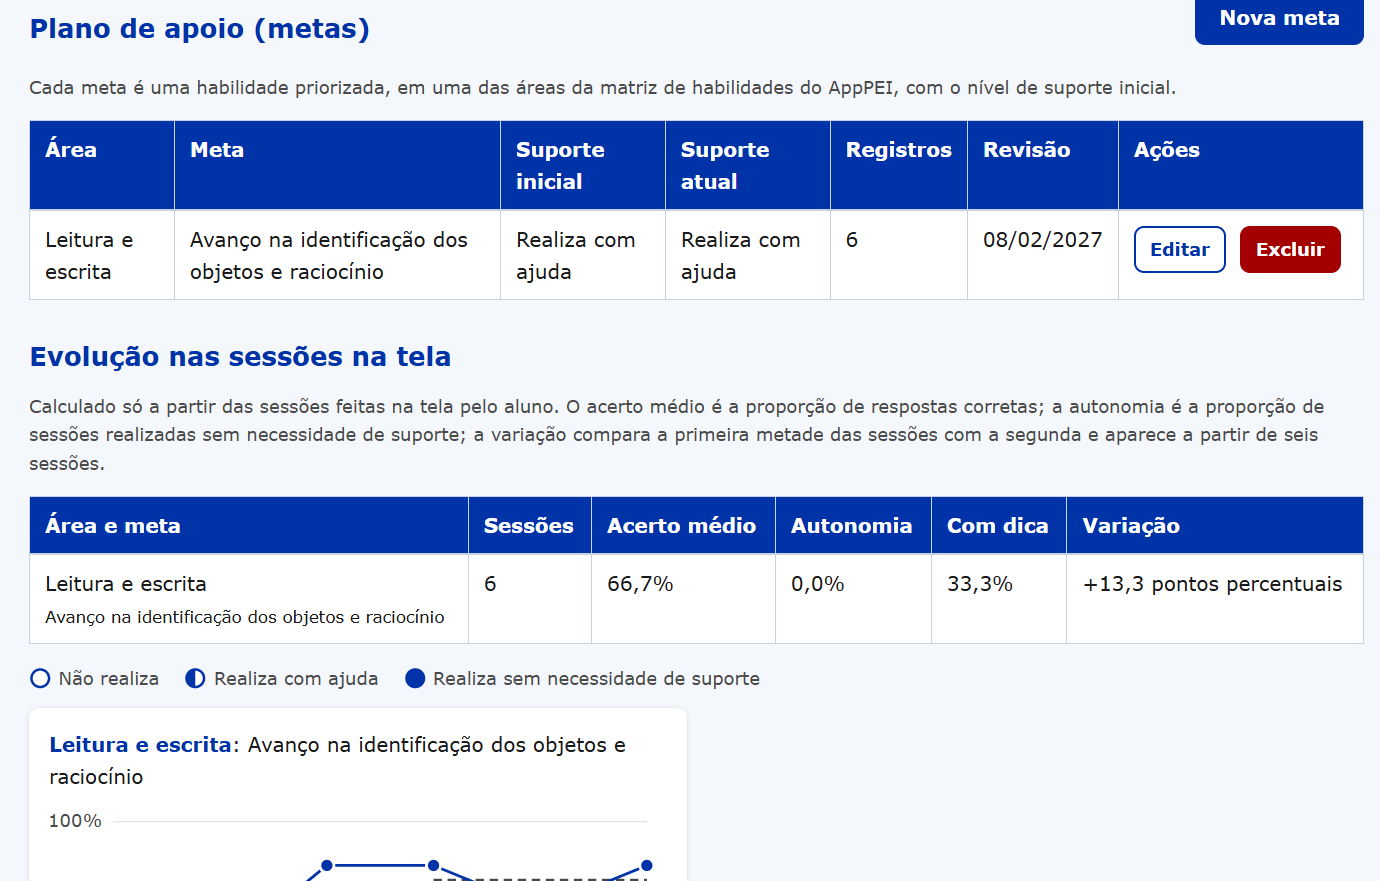
\includegraphics[width=15cm,height=17cm,keepaspectratio]{figuras/figura06-ficha-do-aluno.png}
  \fonte{elaboração própria (2026).}
\end{figure}

\begin{figure}[hbp]
  \legendafig{figure}{Rodada do mini game “Contar e escolher o numeral”}{fig:7}
  % Rodada 2 de 5 do jogo Contar e escolher o numeral até 10: quatro sóis desenhados e botões com os numerais
  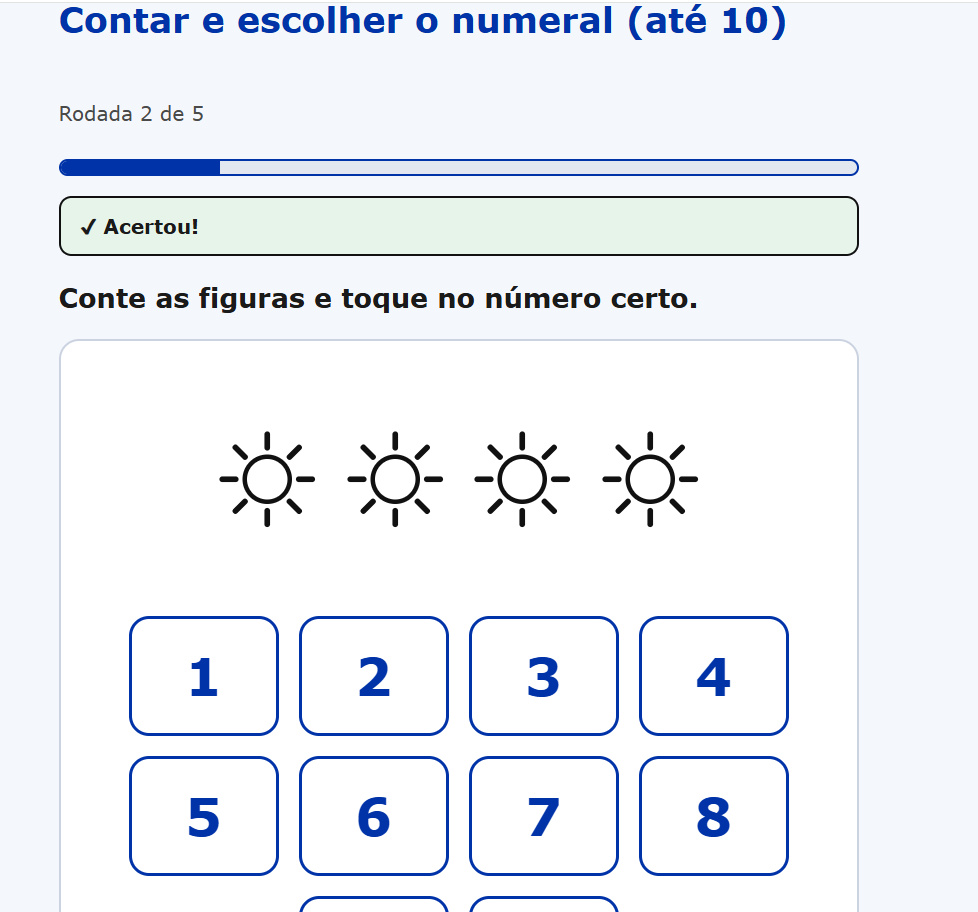
\includegraphics[width=12.9cm,height=10cm,keepaspectratio]{figuras/figura07-rodada.png}
  \fonte{elaboração própria (2026).}
\end{figure}

\begin{figure}[hbp]
  \legendafig{figure}{Escolha dos jogos da sessão, com a meta de cada jogo}{fig:8}
  % Lista de jogos da sessão na ficha do aluno, cada um com a meta em que será gravado; os jogos de áreas sem meta aparecem desabilitados
  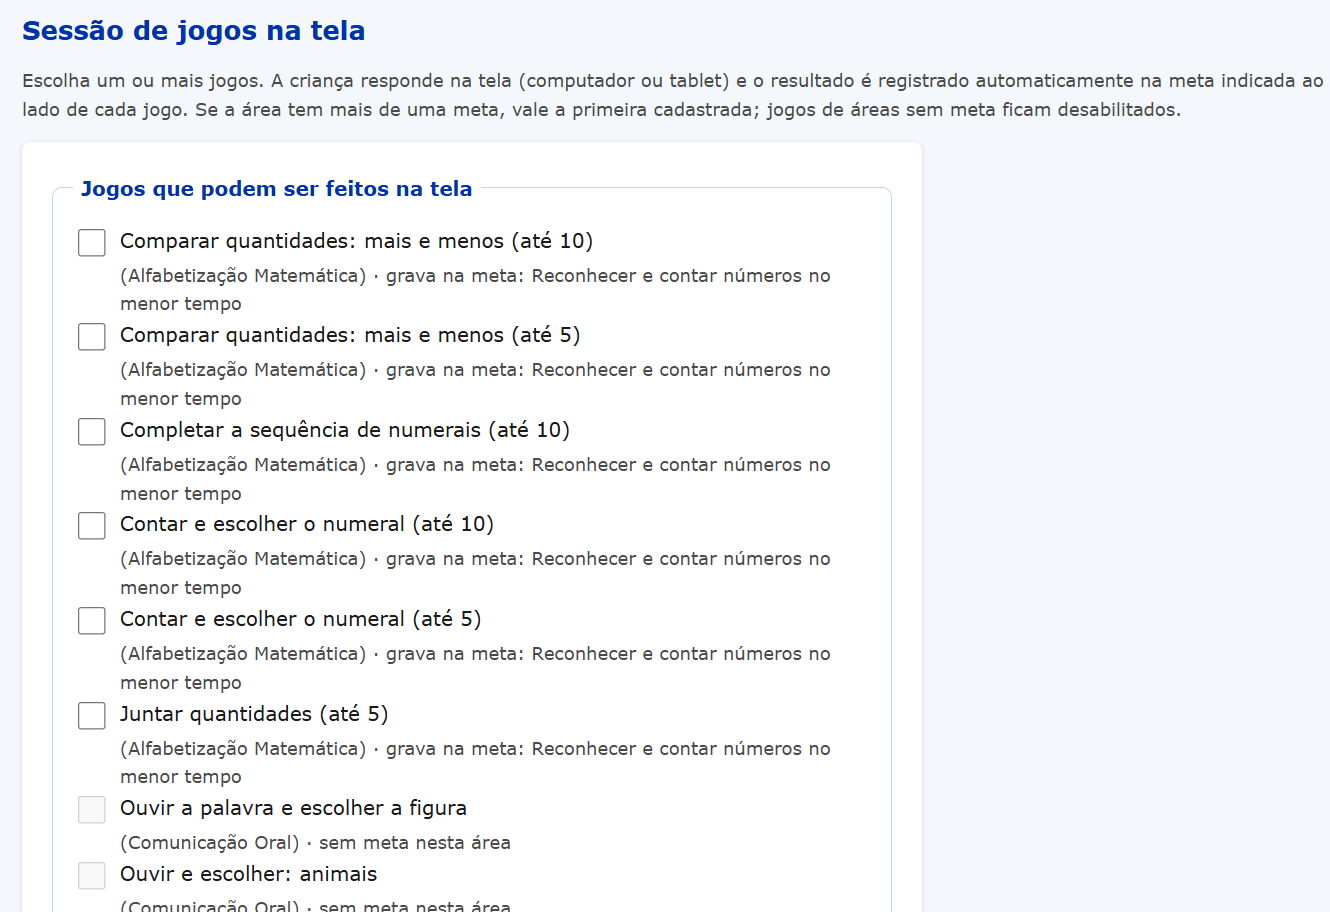
\includegraphics[width=15cm,height=17cm,keepaspectratio]{figuras/figura08-escolha-dos-jogos.png}
  \fonte{elaboração própria (2026).}
\end{figure}

% Gerado de tcc.md (exportado do Claude Docs) por ferramentas/gera_latex.php em 12/11/2026 21:45.
% Para mudar o texto, edite este arquivo; se gerar de novo a partir do documento, as edições feitas aqui se perdem.

\chapter{RESULTADOS E DISCUSSÃO}\label{cap:5}

O UNIA foi concluído como protótipo funcional e passou em todas as verificações técnicas feitas. Este capítulo apresenta essas verificações, compara o sistema com o AppPEI, relata uma avaliação heurística de usabilidade e expõe as limitações, que delimitam o alcance dos resultados.

\section{Verificação técnica}\label{sec:5.1}

A Tabela~\ref{tab:2} resume a verificação descrita na seção~\ref{sec:3.4}.

\begin{tabelacurta}
\setlength{\largtab}{\dimexpr\linewidth-6\tabcolsep-0\arrayrulewidth-1pt\relax}
\legenda{table}{Resultados da verificação técnica}\label{tab:2}\vspace{4pt}
\begin{tabular}{L{0.2655}L{0.3326}L{0.4019}}
\hline
\textbf{Verificação} & \textbf{Escopo} & \textbf{Resultado} \\
\hline
Sintaxe (\textit{php -l}) & Todos os arquivos PHP do sistema & Sem erros \\
Testes automatizados & 63 verificações das regras de negócio & 63 aprovadas, nenhuma falha \\
Conferência das rotas & 45 rotas & Todas apontam para métodos existentes \\
Teste de ponta a ponta & 30 verificações em banco temporário & 30 aprovadas, nenhuma falha \\
Inspeção visual & Ficha do aluno e tela de cada mini game & Sem avisos do PHP e sem rolagem horizontal em tela estreita \\
\hline
\end{tabular}
\fonte{elaboração própria (2026).}
\end{tabelacurta}

O teste de ponta a ponta executou o fluxo principal sobre os modelos e serviços, num banco MySQL temporário, no servidor MariaDB 10.4 do XAMPP, sem passar pelas telas de login. Ele confirmou que o catálogo tem 24 atividades executáveis, seis por área; que um aluno com deficiência auditiva recebe seis sugestões em cada área, exceto em Comunicação Oral, onde os jogos de ouvir não são sugeridos; que seis sessões com acertos crescentes geram, em cada área, seis registros e uma variação positiva; que o histórico do aluno reúne os 24 registros; que as sugestões somem depois que o aluno faz todos os jogos da área; e que a tela de cada um dos 12 formatos é desenhada sem erro.

Esses resultados mostram que o sistema faz o que foi projetado para fazer: mede as respostas, classifica as sessões, separa os resultados por meta e calcula a evolução de forma consistente. Eles não mostram que a medição é válida do ponto de vista pedagógico, isto é, que um aluno classificado como “realiza sem necessidade de suporte” no jogo realiza a habilidade fora dele. Essa pergunta depende de avaliação com professores e alunos, que não foi feita.

\section{Comparação com o AppPEI}\label{sec:5.2}

O Quadro~\ref{qua:10} compara o UNIA com o AppPEI, sua principal referência.

\begin{tabelacurta}
\setlength{\largtab}{\dimexpr\linewidth-6\tabcolsep-4\arrayrulewidth-1pt\relax}
\legenda{quadro}{Comparação entre o AppPEI e o UNIA}\label{qua:10}\vspace{4pt}
\begin{tabular}{|L{0.2381}|L{0.3617}|L{0.4002}|}
\hline
\textbf{Aspecto} & \textbf{AppPEI} & \textbf{UNIA} \\
\hline
Plataforma & Planilha eletrônica do Google & Aplicação web em PHP e MySQL \\ \hline
Foco & Elaboração do PEI & Acompanhamento e medição das metas do PEI \\ \hline
Avaliação inicial & Inventário de habilidades nas quatro áreas, com priorização & Metas por área com nível de suporte inicial; sem inventário completo \\ \hline
Proposta de intervenção & Registrada no plano & Catálogo de atividades com sugestões por meta \\ \hline
Medição do desempenho & Não há & Acerto, dica e tempo em cada rodada \\ \hline
Evolução ao longo do tempo & Não há & Indicadores e gráficos por meta \\ \hline
Documento completo do PEI & Gerado pela ferramenta & Não gerado \\ \hline
Uso em celular ou tablet & Sugestão dos avaliadores & Telas para toque; teste em tablet pendente \\ \hline
Avaliação com usuários & Professores do CAp-UERJ & Ainda não realizada \\ \hline
\end{tabular}
\fonte{elaboração própria (2026), com base em Francisco (2023).}
\end{tabelacurta}

O UNIA não substitui o AppPEI. Faltam a ele o inventário de habilidades usado na avaliação inicial, a matriz completa de priorização e o documento final do plano. O que ele acrescenta está nas etapas em que o AppPEI para: a aplicação das atividades e a avaliação com replanejamento, as duas últimas do ciclo descrito por Francisco (2023). As duas ferramentas podem conviver: as habilidades priorizadas num PEI elaborado no AppPEI podem ser cadastradas como metas no UNIA e acompanhadas sessão a sessão.

O UNIA também responde a parte das sugestões dos professores que avaliaram o AppPEI: trocou a planilha por páginas web, reuniu o acompanhamento numa única ficha por aluno e usa telas pensadas para toque. Em relação à norma, o sistema oferece uma forma concreta de cumprir o que a Portaria MEC nº 421/2026 chama de “estratégias de acompanhamento e de monitoramento do plano” (BRASIL, 2026, art. 11, III). A data de revisão de cada meta, de 90 dias por padrão, é mais frequente que a revisão anual exigida (BRASIL, 2026, art. 7º, § 3º), e a série de sessões dá ao professor os dados para essa revisão.

\section{Avaliação heurística}\label{sec:5.3}

A avaliação heurística é um método de inspeção em que avaliadores examinam a interface à luz de um pequeno conjunto de princípios gerais de usabilidade, as heurísticas, para encontrar seus problemas de usabilidade (NIELSEN, 1994a, p. 152). As telas do UNIA foram inspecionadas, junto com o código das views, segundo as nove heurísticas revisadas por Nielsen (1994a, p. 155), aqui em tradução livre: visibilidade do estado do sistema; correspondência entre o sistema e o mundo real; controle e liberdade do usuário; consistência e padrões; prevenção de erros; reconhecimento em vez de memorização; flexibilidade e eficiência de uso; estética e design minimalista; e ajuda para reconhecer, diagnosticar e corrigir erros. Somou-se a elas a heurística de ajuda e documentação, que fazia parte da lista anterior do autor (NIELSEN, 1994a, p. 156). Cada problema recebeu uma nota de severidade de 0 a 4: 1 indica um problema apenas estético, que só precisa ser corrigido se sobrar tempo; 2, um problema menor, de baixa prioridade; 3, um problema grave, de alta prioridade; e 4, uma catástrofe de usabilidade, a corrigir antes de o produto ser lançado (NIELSEN, 1994b).

A inspeção encontrou pontos que atendem aos princípios. A rodada mostra em que ponto da sessão o aluno está, com o texto “Rodada 3 de 5” e uma barra de progresso, e cada resposta recebe retorno com símbolo, cor e texto; ao final, a ficha do aluno informa os acertos, as dicas e quantos registros foram gravados. A exclusão de alunos, metas e registros e o cancelamento da sessão pedem confirmação, e o cancelamento avisa que nada será registrado. Os formulários mostram no topo um resumo dos erros, com link para cada campo, e as mensagens dizem como resolver o problema, como em “Crie a meta antes de iniciar a sessão”. O vocabulário é o do professor, com estudo de caso, meta e nível de suporte, e textos curtos de ajuda explicam as metas, os indicadores e as sugestões. O Quadro~\ref{qua:11} reúne os problemas encontrados.

\begin{tabelaIFTO}
\setlength{\largtab}{\dimexpr\linewidth-8\tabcolsep-5\arrayrulewidth-1pt\relax}
\begin{longtable}{|L{0.2891}|L{0.2661}|L{0.1549}|L{0.2899}|}
\legendatab{quadro}{Problemas de usabilidade encontrados na avaliação heurística}{qua:11}{4}\\
\hline
\textbf{Princípio} & \textbf{Problema} & \textbf{Severidade} & \textbf{Recomendação} \\
\hline
\endfirsthead
\multicolumn{4}{@{}r@{}}{\textit{(continuação)}}\\
\hline
\textbf{Princípio} & \textbf{Problema} & \textbf{Severidade} & \textbf{Recomendação} \\
\hline
\endhead
\multicolumn{4}{@{}r@{}}{\textit{(continua)}}\\
\endfoot
\fontetab{4}{elaboração própria (2026), com os princípios de Nielsen (1994a) e a escala de severidade de Nielsen (1994b).}
\endlastfoot
Controle e liberdade do usuário; prevenção de erros & Durante o jogo, o menu do professor continua na tela, com a busca e o botão Sair. Um toque da criança tira o jogo da tela, e o Sair encerra o login sem confirmação e descarta a sessão em andamento & 3 & Corrigido: a sessão abre numa tela só com o jogo e o botão Cancelar, que pede confirmação \\ \hline
Prevenção de erros; visibilidade do estado do sistema & Com duas metas na mesma área, a sessão grava o resultado na primeira, e a lista de jogos não mostra em qual meta cada jogo será registrado & 3 & Corrigido: a lista mostra, ao lado de cada jogo, a meta que receberá o resultado \\ \hline
Prevenção de erros & A lista de jogos aceita jogos de áreas sem meta, e o aviso só aparece depois que a sessão começa & 2 & Corrigido: os jogos de áreas sem meta aparecem desabilitados, com aviso \\ \hline
Consistência e padrões & O mesmo objeto se chama ora atividade, ora jogo, inclusive na ficha do aluno, e o PEI aparece nas telas como plano de apoio & 2 & Usar um termo por conceito em todas as telas \\ \hline
Flexibilidade e eficiência de uso & Para comparar o progresso, o professor deve repetir o mesmo jogo, mas o atalho Fazer na tela só aparece para atividades ainda não aplicadas & 2 & Incluir em cada meta um atalho para repetir o último jogo \\ \hline
Estética e design minimalista & A ficha reúne numa página o estudo de caso, as metas, a evolução, as sugestões, a lista de jogos e o histórico, o que exige muita rolagem & 2 & Acrescentar no topo links para cada parte da ficha \\ \hline
Ajuda e documentação & A tela mostra o nível de suporte de cada sessão, mas não explica a regra que o produziu & 2 & Explicar a regra de classificação junto à tabela de evolução \\ \hline
Reconhecimento em vez de memorização & Os valores de cada ponto do gráfico aparecem só ao passar o mouse; no tablet, é preciso buscá-los no histórico & 1 & Mostrar os valores também ao tocar no ponto \\ \hline
Visibilidade do estado do sistema & A última resposta da sessão não recebe retorno na tela: a sessão termina e abre a ficha do aluno & 1 & Mostrar uma tela final com o retorno e uma mensagem de encerramento \\ \hline
Correspondência entre o sistema e o mundo real & A variação aparece em pontos percentuais, termo pouco familiar fora das áreas de exatas & 1 & Acompanhar o número de uma frase simples, como “acertou mais na segunda metade” \\ \hline
\end{longtable}
\end{tabelaIFTO}

Foram encontrados dez problemas: dois graves, cinco menores e três estéticos, e nenhum na categoria de catástrofe. Os dois graves afetavam a confiança no histórico, que é o centro do sistema: um podia interromper a sessão e descartar as respostas, e o outro podia gravar o resultado na meta errada sem que o professor percebesse. Por isso, foram corrigidos logo depois da avaliação: a sessão de jogos passou a abrir numa tela sem o menu do professor, e a lista de jogos da ficha passou a mostrar a meta que receberá cada resultado e a desabilitar os jogos de áreas sem meta, o que resolveu também o terceiro problema do quadro. A regra que define a meta de destino ganhou um teste automatizado. Os demais problemas, menores ou estéticos, tratam de nomes, atalhos e explicações e podem ser corrigidos depois, na ordem da severidade.

A avaliação tem dois limites. Foi feita por um único avaliador, que também participou do desenvolvimento, enquanto Nielsen e Molich (1990, p. 255) desaconselham confiar na avaliação de uma só pessoa e recomendam de três a cinco avaliadores, trabalhando de forma independente; pelo mesmo motivo, as notas de severidade são de uma só pessoa, e Nielsen (1994b) considera satisfatória, para muitos fins práticos, a média das notas de três avaliadores. Além disso, a inspeção aponta problemas prováveis, mas não mostra como professores e crianças de fato usam o sistema, o que depende de testes com usuários.

\section{Limitações}\label{sec:5.4}

As limitações se dividem em três grupos. As de medição e de conteúdo pedagógico são:

\begin{alineasIFTO}
  \item os parâmetros não foram validados: a regra de classificação, as cinco rodadas, as quantidades até 5 ou 10, o mínimo de seis sessões para a variação e os 90 dias de revisão são decisões do protótipo;
  \item as 24 atividades foram propostas neste projeto e ainda não foram avaliadas por profissionais da educação especial;
  \item na área de Comunicação Oral, o sistema mede apenas a compreensão: a criança ouve a palavra e toca na figura, e a produção oral, que exigiria captar a voz da criança, fica de fora;
  \item as figuras são desenhos simples, não testados com crianças, e, se um desenho não for reconhecido, o jogo mede o desenho, e não a habilidade;
  \item a variação mistura os jogos de uma meta, e trocar um jogo fácil por um difícil altera o resultado; para comparar o progresso, o professor deve repetir o mesmo jogo;
  \item uma sessão com vários jogos grava o resultado na primeira meta de cada área, indicada ao lado de cada jogo; se o aluno tem duas metas na mesma área, o professor precisa usar o botão “Fazer na tela” da meta desejada;
  \item as sugestões de atividades são uma regra de ordenação (mesma área, ainda não aplicada, compatível com o tipo de deficiência), e não uma recomendação pedagógica;
  \item o tempo de resposta é gravado, mas ainda não entra nos indicadores nem na classificação.
\end{alineasIFTO}

As de acessibilidade são:

\begin{alineasIFTO}
  \item nenhum mini game atende o aluno com deficiência visual, porque todos dependem de ver as figuras;
  \item não houve auditoria com leitor de tela, ferramenta automática ou usuários;
  \item os detalhes de cada ponto do gráfico aparecem ao passar o mouse, mas não com o toque no tablet.
\end{alineasIFTO}

As técnicas são:

\begin{alineasIFTO}
  \item as telas que exigem login ainda não passaram pelo roteiro de testes manuais do Apêndice B;
  \item o limite de tentativas de login é contado por sessão, e não por endereço, de modo que apagar o cookie reinicia a contagem;
  \item não há limite para pedidos de recuperação de senha;
  \item os modelos usam métodos estáticos, simples de ler, mas difíceis de testar com um banco simulado;
  \item não há migrações de banco: o script de instalação recria o banco e apaga os dados existentes;
  \item o estado da sessão de jogos fica na sessão do servidor, e, se o navegador for fechado no meio, nada é gravado;
  \item as observações do estudo de caso não são criptografadas;
  \item não há testes automatizados de tela.
\end{alineasIFTO}

% Gerado de tcc.md (exportado do Claude Docs) por ferramentas/gera_latex.php em 12/11/2026 21:45.
% Para mudar o texto, edite este arquivo; se gerar de novo a partir do documento, as edições feitas aqui se perdem.

\chapter{CONSIDERAÇÕES FINAIS}\label{cap:6}

Este trabalho desenvolveu o UNIA, um sistema web que apoia o professor no acompanhamento das metas do PEI e mede o desempenho do aluno por meio de mini games. A pergunta de pesquisa era como um sistema web poderia fazer esse acompanhamento medindo o desempenho de forma automática e mostrando a evolução ao longo do tempo. A resposta proposta é ligar cada atividade a uma meta do plano, medir cada resposta na tela e transformar as sessões de uma meta numa série com indicadores e gráficos, usando os mesmos níveis de suporte que o professor já usa para descrever o aluno.

Os objetivos específicos foram atendidos da seguinte forma:

\begin{alineasIFTO}
  \item os elementos do PEI, os níveis de suporte e as exigências das normas de 2025 e 2026 foram identificados no capítulo~\ref{cap:2};
  \item o cadastro de alunos, do estudo de caso e das metas por área, com nível inicial e data de revisão, foi modelado e implementado (seções~\ref{sec:4.1} e~\ref{sec:4.3});
  \item os 12 formatos de mini game, distribuídos em 24 atividades nas quatro áreas do AppPEI, registram acerto, uso de dica e tempo de resposta (seção~\ref{sec:4.4});
  \item a regra de classificação e os quatro indicadores de evolução foram definidos e apresentados em tabela e em gráficos que não dependem de cor (seções~\ref{sec:4.5} e~\ref{sec:4.6});
  \item o sistema passou nas 63 verificações automatizadas e nas 30 verificações do teste de ponta a ponta (seção~\ref{sec:5.1}), e a avaliação heurística apontou dez problemas de usabilidade, dois deles graves, já corrigidos (seção~\ref{sec:5.3}).
\end{alineasIFTO}

A principal contribuição está em aproximar dois grupos de ferramentas que, nas fontes consultadas, aparecem separados: as que organizam o PEI e os jogos que trabalham habilidades. No UNIA, o jogo existe para alimentar a meta, e a meta passa a ter um histórico medido. Isso vai ao encontro das normas recentes, que exigem um PEI com atualização contínua e com estratégias de acompanhamento e de monitoramento. Vai também ao encontro da ideia que motivou o projeto: tornar visível o caminho do aluno da ajuda à autonomia, sessão após sessão.

Os resultados, porém, são técnicos. O sistema funciona como projetado, mas não foi usado por professores nem por alunos, e a regra de classificação, os parâmetros e as atividades são hipóteses do protótipo. A próxima etapa necessária é a validação pedagógica.

\section{Trabalhos futuros}\label{sec:6.1}

Os trabalhos futuros se organizam em três frentes. Na validação:

\begin{alineasIFTO}
  \item avaliar o sistema com professores do AEE e da sala comum, com aprovação de comitê de ética, para validar a regra de classificação, os parâmetros e as atividades;
  \item testar as figuras e os jogos com crianças, com o consentimento dos responsáveis;
  \item fazer uma auditoria de acessibilidade com leitor de tela, ferramentas automáticas e usuários, e repetir a avaliação heurística com três a cinco avaliadores independentes.
\end{alineasIFTO}

Nas funcionalidades:

\begin{alineasIFTO}
  \item tornar a matriz de habilidades editável, como sugeriram os avaliadores do AppPEI;
  \item incluir um inventário de avaliação inicial e gerar o documento do PEI em Portable Document Format (PDF), com o conteúdo mínimo da Portaria MEC nº 421/2026;
  \item criar um relatório para as famílias, que atenda ao registro das devolutivas previsto na mesma portaria;
  \item permitir que vários professores, como o do AEE e o da sala comum, acompanhem o mesmo aluno;
  \item criar mini games para alunos com deficiência visual, baseados em áudio e teclado, além de atividades de arrastar e soltar e de contagem de sílabas;
  \item usar o tempo de resposta nos indicadores e comparar a evolução por jogo e entre metas;
  \item permitir escolher a meta de destino nas sessões com vários jogos e expor o campo de configuração das atividades no formulário de cadastro;
  \item mostrar os detalhes dos pontos do gráfico também pelo toque e corrigir os problemas menores e estéticos da avaliação heurística (Quadro~\ref{qua:11}).
\end{alineasIFTO}

Na parte técnica:

\begin{alineasIFTO}
  \item limitar as tentativas de login por endereço e os pedidos de recuperação de senha;
  \item criptografar os dados sensíveis e definir uma política de retenção;
  \item adotar migrações de banco de dados e testes automatizados de tela.
\end{alineasIFTO}


% =====================================================================================
\postextual
% =====================================================================================
% Gerado de tcc.md (exportado do Claude Docs) por ferramentas/gera_latex.php em 12/11/2026 21:45.
% Para mudar o texto, edite este arquivo; se gerar de novo a partir do documento, as edições feitas aqui se perdem.

\capitulosemnumero{REFERÊNCIAS}

\begin{referenciasIFTO}
ALMEIDA, Fernanda Correia de Lima. \textbf{Plano educacional individualizado}: aplicativo de uso colaborativo na elaboração do PEI para um aluno autista. 2023. 115 f. Dissertação (Mestrado em Educação) – Programa de Pós-Graduação em Educação, Universidade Federal do Tocantins, Palmas, 2023. Disponível em: \url{https://repositorio.uft.edu.br/handle/11612/6107}. Acesso em: 12 nov. 2026.

BENTES, Juliana Ferreira; ARAÚJO, Fabiola Pantoja Oliveira; PIRES, Yomara Pinheiro. ANE - jogos educativos para auxiliar crianças com deficiência intelectual no aprendizado do alfabeto, numerais e emoções. \textit{In}: WORKSHOP DE INFORMÁTICA NA ESCOLA, 26., 2020, On-line. \textbf{Anais} [...]. Porto Alegre: Sociedade Brasileira de Computação, 2020. p. 399-408. DOI: \url{https://doi.org/10.5753/cbie.wie.2020.399}.

BRASIL. [Constituição (1988)]. \textbf{Constituição da República Federativa do Brasil de 1988}. Brasília, DF: Presidência da República, [2026]. Disponível em: \url{https://www.planalto.gov.br/ccivil_03/constituicao/constituicao.htm}. Acesso em: 9 nov. 2026.

BRASIL. Lei nº 9.394, de 20 de dezembro de 1996. Estabelece as diretrizes e bases da educação nacional. \textbf{Diário Oficial da União}: seção 1, Brasília, DF, 23 dez. 1996. Disponível em: \url{https://www.planalto.gov.br/ccivil_03/leis/l9394.htm}. Acesso em: 9 nov. 2026.

BRASIL. Ministério da Educação. Secretaria de Educação Especial. \textbf{Política Nacional de Educação Especial na Perspectiva da Educação Inclusiva}. Brasília, DF: MEC/SEESP, 2008.

BRASIL. Ministério da Educação. Conselho Nacional de Educação. Câmara de Educação Básica. Resolução nº 4, de 2 de outubro de 2009. Institui Diretrizes Operacionais para o Atendimento Educacional Especializado na Educação Básica, modalidade Educação Especial. \textbf{Diário Oficial da União}: seção 1, Brasília, DF, 5 out. 2009.

BRASIL. Decreto nº 7.611, de 17 de novembro de 2011. Dispõe sobre a educação especial, o atendimento educacional especializado e dá outras providências. \textbf{Diário Oficial da União}: seção 1, Brasília, DF, 18 nov. 2011.

BRASIL. Lei nº 13.146, de 6 de julho de 2015. Institui a Lei Brasileira de Inclusão da Pessoa com Deficiência (Estatuto da Pessoa com Deficiência). \textbf{Diário Oficial da União}: seção 1, Brasília, DF, 7 jul. 2015. Disponível em: \url{https://www.planalto.gov.br/ccivil_03/_ato2015-2018/2015/lei/l13146.htm}. Acesso em: 9 nov. 2026.

BRASIL. Lei nº 13.709, de 14 de agosto de 2018. Lei Geral de Proteção de Dados Pessoais (LGPD). \textbf{Diário Oficial da União}: seção 1, Brasília, DF, 15 ago. 2018a.

BRASIL. Ministério da Educação. \textbf{Base Nacional Comum Curricular}. Brasília, DF: MEC, 2018b. Disponível em: \url{http://basenacionalcomum.mec.gov.br/images/BNCC_EI_EF_110518_versaofinal_site.pdf}. Acesso em: 9 nov. 2026.

BRASIL. Decreto nº 12.686, de 20 de outubro de 2025. Institui a Política Nacional de Educação Especial Inclusiva e a Rede Nacional de Educação Especial Inclusiva. \textbf{Diário Oficial da União}: seção 1, Brasília, DF, 21 out. 2025a. Disponível em: \url{https://www.planalto.gov.br/ccivil_03/_ato2023-2026/2025/decreto/d12686.htm}. Acesso em: 9 nov. 2026.

BRASIL. Decreto nº 12.773, de 8 de dezembro de 2025. Altera o Decreto nº 12.686, de 20 de outubro de 2025, que institui a Política Nacional de Educação Especial Inclusiva e a Rede Nacional de Educação Especial Inclusiva. \textbf{Diário Oficial da União}: seção 1, Brasília, DF, 9 dez. 2025b. Disponível em: \url{https://www.planalto.gov.br/ccivil_03/_ato2023-2026/2025/decreto/d12773.htm}. Acesso em: 9 nov. 2026.

BRASIL. Ministério da Educação. Portaria nº 421, de 15 de maio de 2026. Dispõe sobre a Política Nacional de Educação Especial Inclusiva - PNEEI e sobre a Rede Nacional de Educação Especial Inclusiva - Reneei, de que tratam o Decreto nº 12.686, de 20 de outubro de 2025. \textbf{Diário Oficial da União}: Brasília, DF, 18 maio 2026. Texto consolidado, com as alterações da Portaria MEC nº 550, de 18 de junho de 2026.

DENO, Stanley L. Curriculum-based measurement: the emerging alternative. \textbf{Exceptional Children}, [\textit{s. l.}], v. 52, n. 3, p. 219-232, 1985. DOI: \url{https://doi.org/10.1177/001440298505200303}.

DINIZ, Daniele C. S. \textit{et al.} PAR Digital: uma ferramenta web em prol da educação inclusiva. \textit{In}: SIMPÓSIO BRASILEIRO DE SISTEMAS MULTIMÍDIA E WEB, 30., 2024, Juiz de Fora. \textbf{Anais Estendidos} [...]. Porto Alegre: Sociedade Brasileira de Computação, 2024. p. 107-110. DOI: \url{https://doi.org/10.5753/webmedia_estendido.2024.244113}.

DRESCH, Aline; LACERDA, Daniel Pacheco; ANTUNES JÚNIOR, José Antonio Valle. \textbf{Design science research}: método de pesquisa para avanço da ciência e tecnologia. Porto Alegre: Bookman, 2015.

DUTRA, Taynara Cerigueli; MASCHIO, Eleandro; GASPARINI, Isabela. Pensar e Lavar: processo de desenvolvimento e avaliação de um jogo digital educacional para promover o pensamento computacional para crianças neurotípicas e com deficiência intelectual. \textbf{Revista Brasileira de Informática na Educação}, Porto Alegre, v. 31, p. 659-690, 2023. DOI: \url{https://doi.org/10.5753/rbie.2023.3330}.

FARIAS, Ezequiel B.; SILVA, Leandro W. C.; CUNHA, Mônica X. C. ABC Autismo: um aplicativo móvel para auxiliar na alfabetização de crianças com autismo baseado no Programa TEACCH. \textit{In}: SIMPÓSIO BRASILEIRO DE SISTEMAS DE INFORMAÇÃO, 10., 2014, Londrina. \textbf{Anais} [...]. Porto Alegre: Sociedade Brasileira de Computação, 2014. p. 458-469. DOI: \url{https://doi.org/10.5753/sbsi.2014.6136}.

FERNANDES, Marcela Peron. \textbf{Estratégias de gamificação no processo de alfabetização de alunos com Transtorno do Espectro Autista (TEA)}. 2026. 133 f. Dissertação (Mestrado Profissional em Educação Inclusiva) – Faculdade de Ciências e Tecnologia, Universidade Estadual Paulista, Presidente Prudente, 2026. Disponível em: \url{https://hdl.handle.net/11449/320939}. Acesso em: 9 nov. 2026.

FOWLER, Martin. \textbf{Padrões de arquitetura de aplicações corporativas}. Porto Alegre: Bookman, 2006.

FRANCISCO, Priscila Rodrigues Cruz. \textbf{Elaboração do Plano Educacional Individualizado (PEI)}: proposta de um recurso educacional digital. 2023. 146 f. Dissertação (Mestrado Profissional em Ensino na Educação Básica) – Instituto de Aplicação Fernando Rodrigues da Silveira, Universidade do Estado do Rio de Janeiro, Rio de Janeiro, 2023. Disponível em: \url{https://www.bdtd.uerj.br:8443/bitstream/1/20629/2/Disserta%c3%a7%c3%a3o%20-%20Priscila%20Rodrigues%20Cruz%20Francisco%20-%20Completa%20-%202023.pdf}. Acesso em: 9 nov. 2026.

GALDINO, Jaqueline Leite Silva. \textbf{Alfabetização matemática de alunos com TEA}: uma proposta de ensino mediada pela tecnologia. 2024. 77 f. Dissertação (Mestrado em Matemática) – Departamento de Matemática, Pontifícia Universidade Católica do Rio de Janeiro, Rio de Janeiro, 2024. Disponível em: \url{https://www.maxwell.vrac.puc-rio.br/66367/66367.PDF}. Acesso em: 9 nov. 2026.

GIL, Antonio Carlos. \textbf{Como elaborar projetos de pesquisa}. 6. ed. São Paulo: Atlas, 2017.

INSTITUTO NACIONAL DE ESTUDOS E PESQUISAS EDUCACIONAIS ANÍSIO TEIXEIRA (INEP). \textbf{Censo da Educação Básica 2020}: notas estatísticas. Brasília, DF: Inep, 2021. Disponível em: \url{https://download.inep.gov.br/publicacoes/institucionais/estatisticas_e_indicadores/notas_estatisticas_censo_escolar_2020.pdf}. Acesso em: 12 nov. 2026.

INSTITUTO NACIONAL DE ESTUDOS E PESQUISAS EDUCACIONAIS ANÍSIO TEIXEIRA (INEP). \textbf{Censo Escolar da Educação Básica 2024}: notas estatísticas. Brasília, DF: Inep, 2025. Disponível em: \url{https://download.inep.gov.br/publicacoes/institucionais/estatisticas_e_indicadores/notas_estatisticas_censo_da_educacao_basica_2024.pdf}. Acesso em: 12 nov. 2026.

INSTITUTO NACIONAL DE ESTUDOS E PESQUISAS EDUCACIONAIS ANÍSIO TEIXEIRA (INEP). \textbf{Censo Escolar da Educação Básica 2025}: notas estatísticas. Brasília, DF: Inep, 2026. Disponível em: \url{https://download.inep.gov.br/publicacoes/institucionais/estatisticas_e_indicadores/notas_estatisticas_censo_escolar_da_educacao_basica_2025.pdf}. Acesso em: 12 nov. 2026.

MESQUITA, Jeferson Antônio Gonçalves de; BASTOS, Lorena Regina Cruz. Garimpeirinhos: ecossistema digital integrado para alfabetização, inclusão e apoio ao professor. \textit{In}: CONGRESSO BRASILEIRO DE INFORMÁTICA NA EDUCAÇÃO, 14., 2025, Curitiba. \textbf{Anais Estendidos} [...]. Porto Alegre: Sociedade Brasileira de Computação, 2025. p. 200-203. DOI: \url{https://doi.org/10.5753/cbie_estendido.2025.13608}.

MOZILLA. Web Speech API. \textit{In}: MDN WEB DOCS. [\textit{S. l.}]: Mozilla, 2026. Disponível em: \url{https://developer.mozilla.org/en-US/docs/Web/API/Web_Speech_API}. Acesso em: 9 nov. 2026.

NEGRIM, Márcia Regina Corrêa. \textbf{Gestão escolar, docência e tecnologia digital}: trabalho colaborativo para o ensino de alunos com deficiência intelectual. 2019. Dissertação (Mestrado em Docência para a Educação Básica) – Faculdade de Ciências, Universidade Estadual Paulista, Bauru, 2019. Disponível em: \url{https://repositorio.unesp.br/handle/11449/183670}. Acesso em: 12 nov. 2026.

NIELSEN, Jakob. Enhancing the explanatory power of usability heuristics. \textit{In}: SIGCHI CONFERENCE ON HUMAN FACTORS IN COMPUTING SYSTEMS, 1994, Boston. \textbf{Proceedings} [...]. New York: Association for Computing Machinery, 1994a. p. 152-158. DOI: \url{https://doi.org/10.1145/191666.191729}.

NIELSEN, Jakob. \textbf{Severity ratings for usability problems}. [\textit{S. l.}]: Nielsen Norman Group, 1 nov. 1994b. Disponível em: \url{https://www.nngroup.com/articles/how-to-rate-the-severity-of-usability-problems/}. Acesso em: 9 nov. 2026.

NIELSEN, Jakob; MOLICH, Rolf. Heuristic evaluation of user interfaces. \textit{In}: SIGCHI CONFERENCE ON HUMAN FACTORS IN COMPUTING SYSTEMS, 1990, Seattle. \textbf{Proceedings} [...]. New York: Association for Computing Machinery, 1990. p. 249-256. DOI: \url{https://doi.org/10.1145/97243.97281}.

OBJECT MANAGEMENT GROUP. \textbf{OMG Unified Modeling Language (OMG UML)}: version 2.5.1. [\textit{S. l.}]: OMG, dez. 2017. Documento formal/2017-12-05. Disponível em: \url{https://www.omg.org/spec/UML/2.5.1/PDF}. Acesso em: 11 nov. 2026.

OWASP FOUNDATION. \textbf{OWASP Top 10:2021}. [\textit{S. l.}]: OWASP Foundation, 2021. Disponível em: \url{https://owasp.org/Top10/}. Acesso em: 9 nov. 2026.

PAIVA, Willian Micael de; MUNIZ, Raphael de Carvalho; MOREIRA, Irlan Arley Targino; SOUSA, Reudismam Rolim de. Desenvolvimento de um sistema digital para gestão de Planos Educacionais Individualizados (PEIs): promovendo a educação inclusiva por meio de tecnologias. \textbf{Temática}, João Pessoa, ano 22, n. 2, p. 58-82, fev. 2026. Disponível em: \url{https://periodicos.ufpb.br/index.php/tematica/article/view/77906}. Acesso em: 11 nov. 2026.

PRENSKY, Marc. \textbf{Aprendizagem baseada em jogos digitais}. São Paulo: Editora Senac São Paulo, 2012.

PRODANOV, Cleber Cristiano; FREITAS, Ernani Cesar de. \textbf{Metodologia do trabalho científico}: métodos e técnicas da pesquisa e do trabalho acadêmico. 2. ed. Novo Hamburgo: Feevale, 2013.

SILVA, Arthur H. S.; SANTOS, Pedro H.; CUNHA, Mônica X. C. LetraMundo: um jogo sério para alfabetização de crianças com Transtorno do Espectro Autista (TEA) em ambiente escolar. \textit{In}: SIMPÓSIO BRASILEIRO DE INFORMÁTICA NA EDUCAÇÃO, 35., 2024, Rio de Janeiro. \textbf{Anais} [...]. Porto Alegre: Sociedade Brasileira de Computação, 2024. p. 2747-2756. DOI: \url{https://doi.org/10.5753/sbie.2024.244666}.

SOMMERVILLE, Ian. \textbf{Engenharia de software}. 9. ed. São Paulo: Pearson Prentice Hall, 2011.

TANNÚS-VALADÃO, Gabriela; MENDES, Enicéia Gonçalves. Inclusão escolar e o planejamento educacional individualizado: estudo comparativo sobre práticas de planejamento em diferentes países. \textbf{Revista Brasileira de Educação}, Rio de Janeiro, v. 23, e230076, p. 1-18, 2018. DOI: \url{https://doi.org/10.1590/S1413-24782018230076}.

VIGOTSKI, Lev Semenovich. \textbf{A formação social da mente}: o desenvolvimento dos processos psicológicos superiores. 7. ed. São Paulo: Martins Fontes, 2007.

WATT, Adrienne; ENG, Nelson. \textbf{Database design}. 2. ed. Victoria, B.C.: BCcampus, 2014. Disponível em: \url{https://dc.arcabc.ca/_flysystem/repo-bin/2021-10/dc_51320_1.pdf}. Acesso em: 11 nov. 2026.

WORLD WIDE WEB CONSORTIUM (W3C). \textbf{Web Content Accessibility Guidelines (WCAG) 2.1}. [\textit{S. l.}]: W3C, 2018. Disponível em: \url{https://www.w3.org/TR/WCAG21/}. Acesso em: 9 nov. 2026.

\end{referenciasIFTO}

% Gerado de tcc.md (exportado do Claude Docs) por ferramentas/gera_latex.php em 12/11/2026 21:45.
% Para mudar o texto, edite este arquivo; se gerar de novo a partir do documento, as edições feitas aqui se perdem.

\capitulosemnumero{APÊNDICE A \textemdash{} ROTAS DO SISTEMA}\label{ap:A}

O Quadro~\ref{qua:12} lista as rotas definidas no arquivo \textit{config/routes.php}. “Visitante” indica rota acessível apenas sem login, como o próprio login.

\begin{tabelaIFTO}
\setlength{\largtab}{\dimexpr\linewidth-8\tabcolsep-5\arrayrulewidth-1pt\relax}
\begin{longtable}{|L{0.0981}|L{0.3709}|L{0.3585}|L{0.1725}|}
\legendatab{quadro}{Rotas do sistema}{qua:12}{4}\\
\hline
\textbf{Método} & \textbf{URL} & \textbf{Controlador e ação} & \textbf{Acesso} \\
\hline
\endfirsthead
\multicolumn{4}{@{}r@{}}{\textit{(continuação)}}\\
\hline
\textbf{Método} & \textbf{URL} & \textbf{Controlador e ação} & \textbf{Acesso} \\
\hline
\endhead
\multicolumn{4}{@{}r@{}}{\textit{(continua)}}\\
\endfoot
\fontetab{4}{elaboração própria (2026), a partir de \textit{config/routes.php}.}
\endlastfoot
GET & /login & Auth: \textit{formLogin()} & Visitante \\ \hline
POST & /login & Auth: \textit{login()} & Visitante \\ \hline
GET & /cadastro & Auth: \textit{formCadastro()} & Visitante \\ \hline
POST & /cadastro & Auth: \textit{cadastro()} & Visitante \\ \hline
GET & /esqueci-senha & Senha: \textit{formEsqueci()} & Visitante \\ \hline
POST & /esqueci-senha & Senha: \textit{enviar()} & Visitante \\ \hline
GET & /redefinir-senha/\{token\} & Senha: \textit{formRedefinir()} & Visitante \\ \hline
POST & /redefinir-senha/\{token\} & Senha: \textit{redefinir()} & Visitante \\ \hline
POST & /logout & Auth: \textit{logout()} & Logado \\ \hline
GET & / & Home: \textit{index()} & Logado \\ \hline
GET & /perfil & Perfil: \textit{mostrar()} & Logado \\ \hline
POST & /perfil & Perfil: \textit{atualizar()} & Logado \\ \hline
POST & /perfil/senha & Perfil: \textit{alterarSenha()} & Logado \\ \hline
POST & /perfil/excluir & Perfil: \textit{excluir()} & Logado \\ \hline
GET & /atividades & Atividade: \textit{index()} & Logado \\ \hline
GET & /atividades/nova & Atividade: \textit{criar()} & Logado \\ \hline
POST & /atividades & Atividade: \textit{salvar()} & Logado \\ \hline
GET & /atividades/\{id\} & Atividade: \textit{mostrar()} & Logado \\ \hline
GET & /atividades/\{id\}/editar & Atividade: \textit{editar()} & Logado \\ \hline
POST & /atividades/\{id\}/editar & Atividade: \textit{atualizar()} & Logado \\ \hline
POST & /atividades/\{id\}/excluir & Atividade: \textit{excluir()} & Logado \\ \hline
GET & /alunos & Aluno: \textit{index()} & Logado \\ \hline
GET & /alunos/novo & Aluno: \textit{criar()} & Logado \\ \hline
POST & /alunos & Aluno: \textit{salvar()} & Logado \\ \hline
GET & /alunos/\{id\} & Aluno: \textit{mostrar()} & Logado \\ \hline
GET & /alunos/\{id\}/editar & Aluno: \textit{editar()} & Logado \\ \hline
POST & /alunos/\{id\}/editar & Aluno: \textit{atualizar()} & Logado \\ \hline
POST & /alunos/\{id\}/excluir & Aluno: \textit{excluir()} & Logado \\ \hline
GET & /alunos/\{id\}/metas/nova & Meta: \textit{criar()} & Logado \\ \hline
POST & /alunos/\{id\}/metas & Meta: \textit{salvar()} & Logado \\ \hline
GET & /metas/\{id\}/editar & Meta: \textit{editar()} & Logado \\ \hline
POST & /metas/\{id\}/editar & Meta: \textit{atualizar()} & Logado \\ \hline
POST & /metas/\{id\}/excluir & Meta: \textit{excluir()} & Logado \\ \hline
POST & /acompanhamentos/\{id\}/excluir & Acompanhamento: \textit{excluir()} & Logado \\ \hline
GET & /alunos/\{id\}/sessao & Sessao: \textit{iniciar()} & Logado \\ \hline
GET & /sessao & Sessao: \textit{mostrar()} & Logado \\ \hline
POST & /sessao/responder & Sessao: \textit{responder()} & Logado \\ \hline
POST & /sessao/dica & Sessao: \textit{dica()} & Logado \\ \hline
POST & /sessao/cancelar & Sessao: \textit{cancelar()} & Logado \\ \hline
GET & /tipos & TipoDeficiencia: \textit{index()} & Administrador \\ \hline
GET & /tipos/novo & TipoDeficiencia: \textit{criar()} & Administrador \\ \hline
POST & /tipos & TipoDeficiencia: \textit{salvar()} & Administrador \\ \hline
GET & /tipos/\{id\}/editar & TipoDeficiencia: \textit{editar()} & Administrador \\ \hline
POST & /tipos/\{id\}/editar & TipoDeficiencia: \textit{atualizar()} & Administrador \\ \hline
POST & /tipos/\{id\}/excluir & TipoDeficiencia: \textit{excluir()} & Administrador \\ \hline
\end{longtable}
\end{tabelaIFTO}

% Gerado de tcc.md (exportado do Claude Docs) por ferramentas/gera_latex.php em 12/11/2026 21:45.
% Para mudar o texto, edite este arquivo; se gerar de novo a partir do documento, as edições feitas aqui se perdem.

\capitulosemnumero{APÊNDICE B \textemdash{} ROTEIRO DE TESTES MANUAIS}\label{ap:B}

Roteiro para execução no navegador, com dados fictícios e com o banco reinstalado pelo script \textit{database/banco\_acessibilidade.sql}, que apaga os dados existentes.

\begin{conferir}
  \item Importar o script do banco e conferir os 7 tipos de deficiência e as 24 atividades.
  \item Cadastrar um professor com erros de validação e depois com dados corretos; entrar com senha certa e errada; conferir o bloqueio após 5 tentativas.
  \item Recuperar a senha: o e-mail chega, o link redefine a senha e o mesmo link não funciona de novo.
  \item Abrir /alunos sem login: o sistema deve levar ao login.
  \item Com dois professores, conferir que um não abre o aluno, a meta nem o registro do outro (resposta 404).
  \item Pedir dica e cancelar uma sessão: nada pode ser gravado; durante a sessão, o menu, a busca e o botão Sair não podem aparecer.
  \item Abrir cada um dos 12 mini games e conferir se a cena aparece e se os botões respondem ao toque.
  \item No mini game de ouvir a palavra, conferir se a voz fala a palavra (Chrome ou Edge).
  \item Criar metas de matemática e de alfabetização digital, marcar dois jogos na sessão, responder tudo e conferir que nasceram dois registros, um por meta, com o detalhe de cada jogo.
  \item Na lista de jogos da ficha, conferir a meta indicada ao lado de cada jogo e que os jogos de áreas sem meta ficam desabilitados.
  \item No jogo de abrir e fechar o aplicativo, conferir no registro as três etapas e o tempo até abrir.
  \item Repetir a sessão seis vezes na mesma meta e conferir a variação e os gráficos na ficha do aluno.
  \item Excluir um registro do histórico e conferir que ele sai da evolução.
  \item Abrir a sessão num tablet, ou na largura de tablet do navegador, e conferir se os botões são tocáveis.
  \item Criar uma atividade com imagem e fonte, conferir a imagem e excluir a atividade sem perder o histórico do aluno.
  \item Navegar só com o teclado, testar com o leitor de tela NVDA e rodar o Lighthouse.
\end{conferir}


\end{document}
